\documentclass[UTF8,fontset=none,zihao=-4,oneside,openany]{ctexbook}
\usepackage[a4paper,left=22mm,right=22mm,top=24mm,bottom=24mm,headheight=16pt]{geometry}
\usepackage{fontspec}
\setmainfont{TeX Gyre Termes}
\setsansfont{TeX Gyre Heros}
\setmonofont[Scale=0.85]{DejaVu Sans Mono}
\setCJKmainfont{Noto Serif CJK SC}
\setCJKsansfont{Noto Sans CJK SC}
\setCJKmonofont{Noto Sans CJK SC}
\usepackage{amsmath,amssymb,booktabs,array,longtable,tabularx,multirow}
\usepackage{graphicx,caption,subcaption,float}
\usepackage{tikz}
\usetikzlibrary{arrows.meta,positioning,fit,calc}
\usepackage[most]{tcolorbox}
\usepackage{fvextra}
\usepackage{enumitem}
\usepackage{xcolor}
\usepackage{xurl}
\usepackage{fancyhdr}
\usepackage{hyperref}
\usepackage{bookmark}
\definecolor{ink}{HTML}{17324D}
\definecolor{accent}{HTML}{137C8B}
\definecolor{pale}{HTML}{EFF7F8}
\definecolor{softgray}{HTML}{F3F5F7}
\hypersetup{
  colorlinks=true,linkcolor=ink,urlcolor=accent,citecolor=accent,
  pdftitle={Microduck VLM：从预训练到技能微调完整指南},
  pdfauthor={依据本地项目与官方技术资料整理},
  pdfsubject={Qwen3-VL-2B-Instruct、MuJoCo数据采集、QLoRA、技能预测头、评估与部署},
  pdfkeywords={Microduck,Qwen3-VL,VLM,QLoRA,LoRA,技能调用,MuJoCo}
}
\newtcolorbox{notebox}[1]{enhanced,breakable,colback=pale,colframe=accent,
  title={#1},fonttitle=\bfseries\sffamily,boxrule=.5pt,arc=1mm,
  before skip=10pt,after skip=10pt,left=3mm,right=3mm,top=2mm,bottom=2mm}
\newcolumntype{Y}{>{\raggedright\arraybackslash}X}
\newcolumntype{P}[1]{>{\raggedright\arraybackslash}p{#1}}
\setlength{\parindent}{2em}
\setlength{\parskip}{3pt}
\linespread{1.20}
\setlist{topsep=4pt,itemsep=3pt,parsep=0pt,leftmargin=2em}
\setlength{\emergencystretch}{3em}
\renewcommand{\arraystretch}{1.25}
\fvset{breaklines=true,breakanywhere=true,fontsize=\footnotesize,frame=single,
  framesep=2mm,rulecolor=\color{accent},baselinestretch=1.05}
\captionsetup{font=small,labelfont=bf}
\pagestyle{fancy}
\fancyhf{}
\fancyhead[L]{\small\sffamily Microduck 视觉语言技能训练指南}
\fancyhead[R]{\small\thepage}
\fancyfoot[L]{\scriptsize 项目事实快照：2026-11-14 17:14（北京时间）}
\fancyfoot[R]{\scriptsize \nouppercase{\leftmark}}
\renewcommand{\headrulewidth}{.4pt}
\renewcommand{\footrulewidth}{0pt}
\ctexset{
  chapter={format=\Huge\bfseries\sffamily\color{ink},beforeskip=8pt,afterskip=20pt},
  section={format=\Large\bfseries\sffamily\color{ink}},
  subsection={format=\large\bfseries\sffamily\color{accent}}
}
\setcounter{tocdepth}{1}
\begin{document}
\begin{titlepage}
\thispagestyle{empty}
\vspace*{12mm}
{\sffamily\color{accent}\large 实践手册 / 本地 HD1910 仿真项目\par}
\vspace{12mm}
{\sffamily\bfseries\color{ink}\fontsize{31}{42}\selectfont Microduck VLM\par}
\vspace{5mm}
{\sffamily\bfseries\color{ink}\fontsize{23}{34}\selectfont 从预训练到技能微调\par 完整流程与输入输出\par}
\vspace{12mm}
{\large Qwen3-VL-2B-Instruct · 规则示范 · QLoRA · 冻结技能头\par}
\vspace{12mm}
\begin{tikzpicture}[node distance=7mm,>=Latex,
  stage/.style={draw=accent,fill=pale,rounded corners=2mm,minimum width=135mm,
  minimum height=13mm,align=center,font=\sffamily}]
  \node[stage] (a) {公开模型：图像与语言基础能力};
  \node[stage,below=of a] (b) {本地仿真：采集画面、指令、状态和正确技能};
  \node[stage,below=of b] (c) {监督训练：学习下一步技能与参数};
  \node[stage,below=of c] (d) {独立验收：格式、决策、完整机器人任务};
  \draw[->,thick,accent] (a)--(b);
  \draw[->,thick,accent] (b)--(c);
  \draw[->,thick,accent] (c)--(d);
\end{tikzpicture}
\vfill
{\large 阅读目标：理解每一层做什么、数据从哪里来、哪些参数在学习，\\
以及如何判断模型真的能够完成任务。\par}
\vspace{8mm}
{\small 版本 1.0 · 编写日期 2026-11-14\\
本地状态快照 17:14:02（北京时间）；训练进度之后仍会变化。\\
以本地源代码、冻结数据清单及官方论文为依据。}
\end{titlepage}
\frontmatter
\chapter*{怎样使用这本指南}
\addcontentsline{toc}{chapter}{怎样使用这本指南}
如果你第一次接触模型训练，建议依次阅读第1章的全局地图、第2章的预训练基础、第3章的数据和第5章的实际训练。第4章解释机器人如何执行，第6章比较其它训练方案，第7章解释验收，第8章提供操作命令，第9章集中回答常见疑问。目录和来源链接可点击。

本指南中，“当前实现”指 \texttt{/home/luckysir/Strands\_Robots} 内核验过的代码与文件；“公开资料”指文末可追溯的一手模型资料；“建议方案”指可实施但尚未接入的设计；“教学示例”用于解释原理，不冒充真实模型输出。预训练方没有公开的逐条数据、精确配比、全部训练超参数，不可能从本地权重反推出，本书会明确保留这一边界。

学习时可以反复追问四件事：\textbf{输入是什么？输出是什么？谁生成正确答案？哪些参数真的被更新？} 只要这四件事始终清楚，就不会把规则、模型推理、模型训练和底层电机控制混在一起。

\begin{notebox}{本书描述的当前状态}
正式 QLoRA 已在本地运行。固定快照时为第101/2375次参数更新，最新完整检查点为第100步。它还没有完成本轮训练，也没有通过微调后机器人闭环验收。原有 \texttt{serve\_vlm.sh} 仍使用原始 GGUF，尚未自动加载训练中的 LoRA。这里的数字是书面快照，不是实时监控。
\end{notebox}
\tableofcontents
\mainmatter
\chapter{先建立全局地图：谁负责理解，谁负责运动}
\section{你要实现的任务}
小鸭子面对一个包含红、黄、蓝三个球的场景。人可以说“踢红球”“把红色的球踢出去”，也可以说“往后走一点”“左转一下”或“现在看到什么”。球可能在当前视野里，也可能在身后。系统需要看图、理解指令、决定一个动作，执行后重新观察，直到任务结束。

你已有的行走和踢球模型，解决的是身体怎么动。上层视觉语言模型解决的是此刻该选择哪个技能、持续多久、是否需要继续观察。这两部分学习的对象和工作频率不同。把已有底层能力保留下来，可以把本轮实验集中在上层决策。

\begin{figure}[htbp]
\centering
\begin{tikzpicture}[>=Latex,node distance=7mm,
  block/.style={draw=accent,fill=pale,rounded corners=1.5mm,align=center,
  text width=139mm,minimum height=13mm,font=\small\sffamily}]
\node[block] (obs) {观测：front / near 相机、姿态、RGB-D 球位置测量\\用户原始指令 + 最近执行历史};
\node[block,below=of obs] (vlm) {上层决策：预训练 / 微调后的 VLM\\选择一个技能、参数，或输出回答 JSON};
\node[block,below=of vlm] (json) {规定接口：type、skill、seconds、target\_color、reply\\格式校验 + 执行条件检查};
\node[block,below=of json] (low) {底层执行：已有 ONNX 行走 / 踢球策略 + 状态反馈\\MuJoCo 物理仿真，随后恢复站立};
\node[block,below=of low] (new) {重新拍摄、记录反馈、进行下一次上层决策\\独立物理验收判断真实结果};
\draw[->,thick,accent] (obs)--(vlm);
\draw[->,thick,accent] (vlm)--(json);
\draw[->,thick,accent] (json)--(low);
\draw[->,thick,accent] (low)--(new);
\draw[->,thick,accent] (new.east)--++(5mm,0)|-(obs.east);
\end{tikzpicture}
\caption{VLM机器人闭环的总体结构。规则老师另行提供示范，原始采集通过Decision接口执行，导出时才转换为统一五字段标签。一次模型输出只负责下一步。}
\end{figure}

\section{五个阶段的输入和输出}
\begin{longtable}{P{24mm}P{43mm}P{43mm}P{36mm}}
\toprule
阶段 & 输入 & 输出 & 执行者 / 状态\\
\midrule
\endhead
基础预训练与后训练 & 大规模文本、图像、视频及监督或反馈数据 & 已具备视觉语言能力的权重 & Qwen团队；我们下载使用\\
规则示范采集 & 随机场景、语言命令、相机和状态 & 观测、规则动作、执行轨迹、验收结果 & 本机MuJoCo；已完成首批\\
本地监督微调 & 经筛选的观测—目标JSON配对 & LoRA适配器、训练状态、指标 & 本机RTX 4050；正在运行\\
模型推理 & 当前观测、指令、允许的历史与状态 & 动作JSON或含reply的回答JSON & 基础VLM已接通；微调LoRA待接入\\
完整任务评测 & 保留的场景和未参与选模的任务 & 成功率、错误类型、耗时、接触证据 & 微调后闭环尚待完成\\
\bottomrule
\end{longtable}

本地微调不需要重新收集互联网级别的大规模图文数据。它从已有权重出发，学习你的技能接口及场景习惯。相反，直接部署一个未经本地微调的 VLM 也有可能输出合法技能，因为它可以阅读提示词；微调的目的是让这种选择更稳定、更贴合实际，而不是首次赋予它读字的能力。

\section{VLM、VLA、规则与技能库各是什么}
\textbf{VLM（视觉语言模型）}接收视觉和语言信息，输出语言或可被程序解释的结构化内容。本项目中的 Qwen3-VL 本体属于 VLM。

\textbf{VLM 驱动的技能调用系统}把这个模型接到预定义动作接口。模型输出 \texttt{move\_forward} 等技能名和参数，执行器再调用底层策略。动作不是模型输出一串自然语言后随意解释，而是按固定接口严格解析。

\textbf{分层视觉语言动作策略}可以用来描述经过动作示范训练、从视觉和语言预测技能的整套系统。是否称为“分层 VLA”取决于使用的术语习惯；关键是写清楚动作层级。本项目输出的是技能层动作，不是每个电机关节的目标角度或力矩。

\textbf{规则老师}用明确程序逻辑生成下一技能。它不通过梯度更新学习，但可以产生训练示范。\textbf{技能库}则给出了动作名称、执行接口、约束和已有控制器。它不是一段“让模型想象鸭子如何运动”的文字。

\begin{notebox}{“固定技能”不等于“固定整段任务”}
左脚踢球的底层动作已经训练好；但是走向哪个球、什么时候转身、如何接近、何时踢球，仍可根据每次新画面改变。你需要学习的主要是这些技能之间的选择与切换。
\end{notebox}

\section{训练、推理和物理控制是三个不同的时钟}
训练中的一次更新，在当前机器上约需22秒，处理四条已经保存的样本。此时不要求真实机器人同步运动，主要工作是计算损失和梯度。

推理中的一次决策，消耗的是看当前图像并生成输出的时间。它可能随着模型、后端、输入长度和显卡状态改变。训练一次更新的22秒不能直接当作部署时一次技能决策的延迟。

底层控制以较高频率读取身体状态并给出关节动作。当前策略控制约50Hz、物理仿真步频200Hz。上层模型等待时仍须维持站立；不能等每个语言token出来才给电机一次指令。

\section{“模型知道什么”的四个来源}
\begin{enumerate}
\item \textbf{预训练权重}：学到图像、词语、颜色、空间关系和语言表达等统计规律；不保证天然理解这只鸭子的精确踢球坐标。
\item \textbf{本次提示词}：列出九个技能、动作参数、坐标方向和输出五个字段。模型通过阅读上下文获知当前接口。
\item \textbf{当前观测和指令}：用户说“红球”，两路相机和辅助测量提供可见球的信息。目标颜色来自原始指令及对话上下文。
\item \textbf{本地示范训练}：把典型输入与合适的技能选择关联起来，更新LoRA或未来的技能预测头。
\end{enumerate}
这也解释了“没有微调，怎么知道技能库”：知道接口可以依靠提示词；稳定掌握接口在复杂场景下的正确使用，需要实际数据和验证。格式由程序设计者规定，模型学习或遵循这个协议。

\section{三个“成功”必须分别记录}
\begin{longtable}{P{31mm}P{54mm}P{66mm}}
\toprule
成功的层次 & 能说明什么 & 不能直接说明什么\\
\midrule
\endhead
训练程序成功运行 & 前向、反向、优化器更新和检查点保存正常 & 小鸭子已经会踢指定球\\
离线输出匹配示范 & 在给定画面下生成的格式、技能或参数符合标签 & 自己行动后仍能完成完整任务\\
闭环物理任务成功 & 从起点出发，实际搜索、接近、踢中目标并站稳 & 任意新场景、真实机器人和所有新说法都能成功\\
\bottomrule
\end{longtable}
后面每个章节都会保留这三个层次。特别是规则老师的277/300随机踢球成功率，是采集质量证据，不能写成微调后VLM的成功率。

\section{本轮实验的边界}
目前覆盖的是固定三色球、已有九种技能、有限范围随机布局，以及相应移动和视觉问答。拾布、张嘴发声、真实语音识别、麦克风和实体机器人部署，不属于这次已完成的数据与验证范围。“现在能看到什么”的示范主要描述本场景中的球，也不能据此宣称已验证开放世界视觉问答。

这是一轮可复现的起点。保留失败记录、区分训练与测试、说明哪些输入来自辅助测量，比用一个好看的损失数值宣称全部学会更有助于判断下一步该改数据、改提示词，还是改模型。

\chapter{预训练 VLM 从哪里来，它究竟在计算什么}

\section{先分清三个时间阶段}

你现在使用的 \texttt{Qwen3-VL-2B-Instruct} 是已经完成通用训练、能够接受图像和文字的模型。本地微调从这些已有权重出发。为了理解后续每个文件和命令，先把时间轴分成三段：

\begin{enumerate}
\item \textbf{厂商训练基础模型。} 大量通用数据决定它怎样把图像与语言联系起来，以及怎样理解问题、生成回答。这些训练发生在我们下载模型之前。
\item \textbf{我们做机器人任务微调。} 使用相机画面、语言任务、状态和示范动作，让已有模型适应小鸭子的技能定义及执行条件。这是当前正在进行的 QLoRA 监督微调。
\item \textbf{部署后进行推理。} 把新画面和新指令交给模型，生成一次决策，执行后再观察。普通推理不会更新权重；连续走了十步，也不意味着自动训练了十次。
\end{enumerate}

这里的“预训练模型”是从使用者角度说的：它是我们任务训练的起点。具体下载的 Instruct 检查点还包含厂商的指令后训练，不能把它理解为只学过下一词预测、完全没学过对话的原始模型。官方提供 Instruct 与 Thinking 等版本；本项目使用前者。\cite{qwen-card}

\begin{notebox}{一个必须明确的边界}
会识别“球”、理解“红色”和“向左”，不等于知道 HD1910 的每个关节该转多少，也不等于知道本项目 \texttt{kick\_left} 的参数和前置条件。技能库由本项目提供；底层动作由已有控制器执行。通用视觉语言知识、上层技能决策、底层运动控制是三个相互配合的部分。
\end{notebox}

\section{模型名称、文件与参数分别表示什么}

\texttt{Qwen3-VL} 是模型家族；VL 指视觉与语言；\texttt{2B} 是规模档位名称，不能简单地用“2B 乘每参数字节数”代替完整显存预算；\texttt{Instruct} 表示面向指令交互的版本。模型卡将它归类为图像加文本到文本的模型，并标注 Apache-2.0 许可证。本地调用无需按每次请求向 API 服务商付费，但设备、存储和电力仍有成本；采用云端服务时计费由具体服务决定。\cite{qwen-card}

“权重”是一大组训练得到的数值，保存着模型所学的统计规律。“配置”规定层数、维度等结构；“Tokenizer”规定文字如何分成 token；“Processor”还处理图片及聊天模板。因此，仅有一个权重文件并不等于已经拥有正确的完整输入管线。

本地下载的配置与官方 2B 配置一致：语言部分有 28 层、隐藏维度 2,048、词表大小 151,936；视觉部分有 24 层、隐藏维度 1,024，输入为 3 个颜色通道，图像 patch 大小为 16，空间合并系数为 2。配置中的最大位置长度为 262,144；这是结构支持值，不代表本机能按这个长度训练。本次本地训练的上下文上限是 4,096。\cite{qwen-config}

\section{从一张图片到一句回答}

\subsection{第一步：把人类输入整理为消息}

人类看到的是“这张图里有什么？”和一张图片。程序看到的是一组有角色的消息：\texttt{system} 给出任务约定，\texttt{user} 提供图像和问题，\texttt{assistant} 是模型要生成的回答。一个用户消息可以包含多个图像块和文本块。Processor 负责聊天模板、文字分词和图像预处理。\cite{multimodal-template}

下面是教学用伪结构，帮助理解数据方向，并不是复制即可运行的模型调用代码：

\begin{Verbatim}[breaklines=true,fontsize=\small]
messages = [
  {role: "system", content: [task_and_output_rules]},
  {role: "user", content: [front_rgb, near_rgb, instruction, state]}
]
processed = processor(messages)
answer_tokens = model.generate(processed)
answer_text = tokenizer.decode(answer_tokens)
\end{Verbatim}

训练时还会附加已知的正确 assistant 回答；推理时只给到 assistant 应该开始回答的位置。两者输入格式要对齐，否则模型训练时见到的分布与实际执行时不同。

\subsection{第二步：图片变成视觉特征}

模型并不是先把图片完整地翻译为一句中文再思考。它会把像素整理为小块，让视觉编码器计算一组数值向量。例如，一个向量可能携带局部颜色、边缘、纹理与物体关系等混合信息；不能把每个维度都直接解释成一个人类概念。

Qwen3-VL 的主要组成是视觉编码器、视觉与语言之间的合并／投影模块以及语言模型。系列报告说明，2B 和 4B 使用 SigLIP2-Large 作为视觉编码器基础；视觉特征经空间合并后进入语言模型。\cite{qwen-report} 合并与投影的作用，可以理解为把视觉侧的数值表示变成语言侧能利用的表示。维度匹配只是必要条件，跨模态训练还要让这些表示具有可用的对应关系。

“视觉 token”与“文字 token”不能混为一谈。文字 token 有词表编号，可以解码为文字片段；视觉 token 通常是从图片计算出的向量序列。二者在多模态上下文中相互作用，并不表示每块图片都必定对应某个汉字。

Qwen3-VL 还通过 DeepStack 将不同深度的视觉特征融入语言层，使用交错式 MRoPE 表达空间／时间位置，并通过文字时间戳处理视频时间关系。这些是模型家族的结构能力。\cite{qwen-repo} 当前小鸭子每次提交的是两张观察图片，不能因为基础模型支持视频，就把当前管线说成已经输入连续视频。

\subsection{第三步：数值张量进入模型}

典型预处理结果包含以下几类对象。它们不是四份独立答案，而是一次模型计算需要的输入。\cite{multimodal-template}

\begin{longtable}{P{4.0cm}P{10.5cm}}
\textbf{名称} & \textbf{通俗含义} \\
\hline
\texttt{input\_ids} & 文字及特殊占位标记的整数序列；每个整数是一个 token 编号。\\
\texttt{attention\_mask} & 告诉模型哪些位置有效，哪些只是批处理填充。\\
\texttt{pixel\_values} & 图片经缩放、归一化、分块等处理后的像素张量。\\
\texttt{image\_grid\_thw} & 视觉网格的时间、高、宽结构，供位置及视觉序列组织使用。\\
\end{longtable}

同一张图片的原始像素、视觉特征、最后输出的 token 是三个不同层级。原始 RGB 通常是三通道颜色值；隐藏状态是一组浮点向量；最终输出则是可以解码为文字的词表编号。图片分辨率、图片数量、提示词和历史长度都会改变一次计算的工作量。

\subsection{第四步：逐个生成输出 token}

语言模型根据当前全部输入以及已经生成的回答前缀，计算下一个 token 的分数，归一化后得到概率分布。选择一个 token、接到回答后面，再继续下一次预测，直到结束标记或达到生成长度限制。官方推理接口最终把生成的编号解码为文本。\cite{qwen-transformers}

如果回答是“前面有一个红球”，模型并不是从固定句子表里一次挑中整句；如果回答是 JSON，它同样要逐段生成括号、键名、值和标点。一个动作名称可能由多个 token 组成，不能假设 \texttt{move\_forward} 必定只占一个 token。

\section{预训练到底怎样让模型学会看图说话}

\subsection{用一个简化样本理解学习过程}

设训练样本包含“一张桌面上放着红球的图片”，以及目标描述“桌面上有一个红色的球”。这只是自造的教学示例，不是对官方真实训练样本的转述。

训练会让模型在看到图片和前文后，依次预测正确描述中的 token。假设应输出“红”，但模型给“蓝”的概率更高，损失就会较大。反向传播计算哪些可训练参数使这个错误更严重，优化器再小幅调整它们。很多不同图片、不同语言表达、不同问题反复出现后，模型逐渐建立可迁移的视觉与语言联系。

用公式表示一种典型自回归目标：
\[
  L=-\frac{1}{T}\sum_{t=1}^{T}\log p_{\theta}
  \left(y_t\mid x,y_1,\ldots,y_{t-1}\right).
\]
其中，$x$ 是图像和文字条件，$y_t$ 是第 $t$ 个目标 token，$\theta$ 是当前可训练参数，$T$ 是参与计算损失的目标长度。正确 token 的概率越高，对应损失越低。这是用于理解的基础表达式；官方大规模训练可能采用不同样本权重、数据配比和更复杂目标，不能把这个简式当成其完整复现配方。

监督训练通常使用正确的回答前缀，即 teacher forcing。训练预测到“红色”时，前面已经给出正确文字；自由生成时，前文是模型自己刚生成的文字。于是，“正确前缀条件下的验证损失降低”与“自己完整生成的回答可靠”并不等价。这也是我们既要计算验证损失，又要做自由生成和仿真闭环测试的原因。

\subsection{官方公开了哪些阶段}

下面仅压缩列出系列技术报告公开的预训练设置，B 表示十亿、T 表示万亿 token；token 预算不是图片张数。\cite{qwen-report}

\begin{longtable}{P{1.1cm}P{4.0cm}P{3.0cm}P{2.4cm}P{2.4cm}}
\textbf{阶段} & \textbf{目的} & \textbf{更新部分} & \textbf{token 预算} & \textbf{序列长度}\\
\hline
S0 & 视觉语言对齐 & 合并／投影层 & 67B & 8,192\\
S1 & 多模态预训练 & 全部组件 & 约 1T & 8,192\\
S2 & 长上下文学习 & 全部组件 & 约 1T & 32,768\\
S3 & 超长上下文适配 & 全部组件 & 100B & 262,144\\
\end{longtable}

对齐阶段可理解为先让已有视觉能力和语言能力连得起来；后面的联合训练进一步调整它们的协作方式；更长上下文训练让模型有机会学习跨度更大的依赖。这个解释说明每个阶段要解决的问题，并不意味着你的 6GB 显卡需要重做厂商的全部流程。

\subsection{用过什么数据，哪些细节仍不知道}

系列报告列举的类型包括图像描述、图文交错网页／文档、视觉问答、OCR、定位与计数、空间与三维标注、代码、视频、GUI／工具使用，以及纯文本。定位数据举例包含 COCO、Objects365、OpenImages、RefCOCO 和 PixMo；数据还包含内部采集及合成内容。\cite{qwen-report}

可以用下面这些\textbf{自造教学样本}理解各类监督信号的差别：

\begin{longtable}{P{3.0cm}P{6.0cm}P{5.3cm}}
\textbf{任务类型} & \textbf{输入示例} & \textbf{目标输出示例}\\
\hline
图像描述 & 一张桌面照片 & “桌上有红球和蓝杯子。”\\
视觉问答 & 图片＋“球是什么颜色？” & “红色。”\\
文字识别 & 一张标牌照片 & 标牌上可见的文字。\\
视觉定位 & 图片＋“指出红球的位置” & 目标点或边界框坐标。\\
关系判断 & 图片＋“球在杯子的哪一侧？” & “在杯子的左侧。”\\
视频理解 & 一段带时间信息的画面＋问题 & 事件描述或对应时间段。\\
工具调用 & 观察＋任务＋可用工具说明 & 某个工具名称及参数。\\
机器人技能监督 & 两路图＋任务＋状态＋历史 & 本项目下一步技能的 JSON。\\
\end{longtable}

前几类能力能帮助理解机器人场景，但最后一行仍需要本项目定义。即使通用数据中有工具调用任务，模型也不能凭空获知一套尚未展示给它的私有工具接口。

\begin{notebox}{公开资料的范围}
官方系列报告不是当前 2B-Instruct 检查点逐样本、逐轮次的训练清单。公开的类别和阶段设置不能反推出每个小模型见过的所有样本、精确比例、随机顺序或全部过滤阈值。因此不能声称它预训练时看过我们的 HD1910、已学过我们的踢球控制器，或给出没有公开依据的完整数据配方。
\end{notebox}

\section{Instruct 是怎样在预训练后形成的}

系列技术报告的后训练流程包含监督微调（SFT）、强模型到弱模型的知识蒸馏以及强化学习（RL）；标准回复与显式推理格式的数据面向不同版本。\cite{qwen-report} 这些概念分别解决不同问题：

\begin{itemize}
\item \textbf{SFT：学习示范。} 给定问题和目标回答，用目标回答监督模型。你当前的机器人训练也采用这一基本形式，只是示范来自任务规则和仿真记录。
\item \textbf{蒸馏：学习更强教师的行为。} 教师可以提供答案或概率信息，学生学习模仿其中有用的能力。教师是规则程序时，通常更直接称为示范模仿；不应自动宣称使用了厂商相同的蒸馏算法。
\item \textbf{RL：依据奖励改变策略。} 训练中生成候选行为，依据可验证结果或其他奖励信号优化。保存失败案例本身不是 RL；必须把奖励与参数更新过程实际连接起来。
\end{itemize}

厂商用过 RL，不意味着我们现在也在跑 RL；我们接着一个经历过多阶段训练的基础模型，用自己的监督样本进行 QLoRA。SFT 描述学习信号，QLoRA 描述参数更新与存储方式，两者可以同时成立。

\section{它的输出格式究竟由谁决定}

基础模型的自然输出是文本 token 序列，没有天生绑定我们五字段的机器人 JSON。固定格式来自几层约束的共同作用：

\begin{enumerate}
\item \textbf{系统提示} 告诉模型可用技能、各参数的意义，以及只能生成什么格式。
\item \textbf{微调样本} 反复示范相同格式和合理决策，使输出更符合任务。
\item \textbf{解码约束（如果实际启用）} 限制可生成的语法结构；本次不能把“提示要求 JSON”自动说成实现了强制语法解码。
\item \textbf{程序解析和守卫} 检查 JSON 字段、范围和当前执行条件。格式正确仍可能选错技能，因此执行前还要检查动作是否允许。
\end{enumerate}

例如，下列是本项目协议的一种教学示例，而不是该基础模型原生保证的输出：

\begin{Verbatim}[breaklines=true,fontsize=\small]
{
  "type": "skill",
  "skill": "move_forward",
  "seconds": 0.2,
  "target_color": "red",
  "reply": ""
}
\end{Verbatim}

“红色”来自用户目标与场景观察之间的关联：指令确定想找哪种球，图像及测量确定哪一个球在哪里。技能定义来自程序提供的提示与训练示范。输出格式来自项目协议，模型学习遵守它；最终是否执行由程序决定。

这一结构当前最清楚的叫法是“VLM 驱动的技能调用”。经过机器人动作示范训练后，也可按动作层级称为“分层视觉语言动作策略”。名称不是验收指标：真正要检查的是输入里有什么、输出是什么、哪些参数被更新，以及闭环任务是否成功。

\chapter{仿真、规则示范与真实训练数据}
\label{chap:data}

本章说明训练数据究竟怎样产生、什么可以交给模型、什么只能用于验收。这里的数据来自本机 HD1910 小鸭子仿真中的实际执行记录。既没有让大模型凭空编造动作答案，也没有把“发出踢球命令”自动当成“踢球成功”。全文中的采集数量与样本均取自已经冻结的正式数据集。

\section{仿真里的小鸭子与三个球}

场景由 \texttt{scene.py} 读取本地 Microduck 的 \texttt{scene\_ball.xml} 后生成。机器人有可移动、可转动的自由基座，躯干主体名为 \texttt{trunk\_base}。底层策略控制 14 个关节：每条腿各有髋偏航、髋侧摆、髋俯仰、膝、踝，共 10 个；颈俯仰及头部俯仰、偏航、侧摆，共 4 个。嘴部不在当前 14 维控制输出中，所以这轮技能训练并没有实现“张嘴叫两声”或“叼布”。

动力学使用 CPU MuJoCo；\texttt{load\_scene(...,"hd1910")} 加载本地 HD1910 参数文件 \texttt{1910\_m6.json}，通过 BAM 执行器模型把关节目标变成力矩。记录中的 \texttt{actuator=sts3215} 是这套模拟实现的模型名称，不能据此认定实体机器人的实际舵机型号。当前名义配置为 5\,ms 物理步长、4 个物理步的命令延迟，即 20\,ms；电压、压降和延迟固定，不进行这部分的域随机化。它也不是原先 GPU/Warp 训练环境的逐位复现。

红、黄、蓝三个球都能在物理世界中运动、碰撞；球半径为 0.035\,m，场景为灰色棋盘地面。主集合随机抽取距离 0.3--0.6\,m、方位覆盖一整圈的位置，球之间至少相隔 0.20\,m。这里先均匀采样半径、再均匀采样角度，并非在圆环面积上均匀采样。复位时机器人躯干初始高度 0.12\,m，关节置于已有策略的 HOME 姿态，先执行 2\,s 站立，再开始任务记录。

球的位置、相机和接触都由同一个物理场景产生；踢球效果不是播放一段角色动画，也不是直接修改球坐标来假装踢中。实际关节目标、接触力、球运动与身体倾斜都有轨迹记录。

\section{两台虚拟相机：看到什么、装在哪里}

两台相机均由本项目额外添加，固定在 \texttt{trunk\_base} 上，不随头部关节单独转动。坐标是相对躯干的安装位置：$+X$ 朝前、$+Y$ 朝左、$+Z$ 朝上，单位为米。它们不是离地高度，也不是世界坐标。

\begin{longtable}{P{2.0cm}P{4.0cm}P{2.4cm}P{6.1cm}}
\hline
名称 & 躯干相对位置 & 俯视角／竖直视场 & 用途\\
\hline
\endhead
\texttt{front} & $(0.14,0,0.16)$ & $45^\circ/85^\circ$ & 朝前下方观察，用于发现远一些的球及接近过程。\\
\texttt{near} & $(0.17,0,0.12)$ & $110^\circ/90^\circ$ & 朝下并向后观察脚边，用于球已经接近身体后的精细对齐；会看见机器人自身。\\
\hline
\end{longtable}

代码中的俯视角以水平方向为起点，因此 $90^\circ$ 是正下方，$110^\circ$ 是越过正下方再朝后 $20^\circ$。近场相机解决的是前置相机脚边盲区；它是当前实验的虚拟传感器配置。以后若实体只有一台相机，需要重新确定安装位姿或调整方案，不能把双相机训练结果直接当成单相机能力。

每次观察先冻结一份物理状态，再从该状态渲染两幅 $320\times240$ 的 RGB，以及各自对齐的深度图。RGB 是 \texttt{uint8} 三通道图像；深度是以米为单位的光轴方向距离，保存为浮点数组。深度不是普通 RGB 的第四个颜色通道。仿真深度没有在这轮采集中加入真实深度相机的空洞和噪声。

\begin{figure}[htbp]
\centering
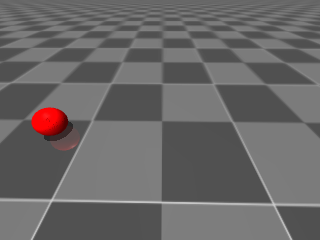
\includegraphics[width=.47\linewidth]{assets/sample_front.png}\hfill
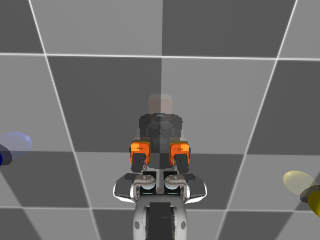
\includegraphics[width=.47\linewidth]{assets/sample_near.png}
\caption{真实训练首样本的 front（左）与 near（右），seed=1000，同一时刻。原指令为“现在能看到什么？”。这是机器人实际输入视角，未使用外部观察相机。}
\end{figure}

交互窗口左边的第三人称画面方便人观察机器人，右边显示 front 和 near。第三人称画面不送给 VLM，也不进入这次训练样本。训练实际输入的是两幅 RGB，另附 RGB-D 检测所得的结构化测量，而不是把整张深度图送进 Qwen 图像编码器。旧的 \texttt{dataset.py} 还保留过 RGB-only 导出接口；本轮正式数据使用新的 \texttt{training\_data.py}，不能用旧文件的简介推断当前输入。

\subsection{球的三维位置从哪里来}

\texttt{perception.py} 先按 RGB 通道阈值分别找红、黄、蓝区域，取至少 10 个像素的连通区域，再把像素和对应深度反投影成点云。它用已知球半径 0.035\,m 拟合球面，并检查曲率、内点比例、残差和可见球面的几何跨度，避免把一块同色地板误当成球。拟合中心通过相机安装旋转和平移变换到躯干坐标系。

检测记录包含颜色、球心 \texttt{center\_body\_m}、像素中心 \texttt{pixel\_uv}、拟合内点数 \texttt{pixels}、拟合残差 \texttt{fit\_residual\_m}、来源相机和 \texttt{confidence}。最后一个值是几何质量分数，并不是“有 90\% 概率正确”这样的校准概率。两台相机同时检测到同色球时，保留质量较高的一项；当前任务假设每种颜色只有一个球。

这条测量链没有读取球的世界坐标或物体分割 ID。不过它依赖颜色、球体形状和已知半径的先验，不能被称作“任意物体的通用识别”。身体的 yaw、倾角和静止判断则来自仿真状态，作为本体传感器的代理；迁移到实机时，需要相应的姿态和速度估计。应明确区分“没有把球的真值位置交给模型”和“输入完全没有仿真状态”。

本节核对：\texttt{scene.py}:10--75；\texttt{runtime.py}:23--44、51--119、281--334；\texttt{perception.py}:89--183。

\section{规则老师怎样选下一步}

采集时使用 \texttt{RuleVLMBackend} 处理语言与视野描述，再由 \texttt{KickPlanner} 处理踢球。虽然类名包含 VLM，它是一个规则接口实现，没有预训练神经网络参与这些示范。它根据本次 RGB-D 测量、机身状态和自身少量记忆，一次选择一个短动作；实际执行后重新看图，再决策。

下面给出真实优先级。前面的条件成立后就立即返回动作，因此不是把所有条件同时执行。

\begin{longtable}{P{2.2cm}P{8.0cm}P{4.4cm}}
\hline
阶段 & 真实判断 & 返回动作\\
\hline
\endhead
搜索 & 当前没有目标颜色。只在搜索期间累计包裹处理后的 yaw 变化，计算已覆盖角度范围。覆盖达到 $2\pi+0.25$\,rad 后仍不可见，则结束为未找到。 & \texttt{turn\_left}，1.0\,s；发现目标后清空搜索角度记录。\\
转向目标 & 球距躯干平面距离 $>0.24$\,m，或者球的 $x<0.03$\,m，且方位角绝对值 $>0.35$\,rad。 & 按角度符号左转或右转，0.6\,s。\\
选择并锁脚 & 首次满足目标 $x<0.24$\,m 时，$y\geq0$ 锁定左脚，否则锁定右脚。 & 保存内部脚别；后续使用该脚对应目标点。\\
站稳与踢球 & 球心与脚目标点的 $x,y$ 误差分别不超过 0.012\,m。首次对齐或身体未静止时先等待。 & 真正的对齐站立 0.6\,s；再次确认后踢对应脚 0.5\,s。\\
避开干扰球 & 还需前进，另一色球位于前方且 $x<\min(x_{\rm target},0.24)$、$|y|<0.10$\,m。 & 向该干扰球的反侧平移 0.32\,s。\\
横向对齐 & 远处 $x>0.24$\,m 时横向容差 0.05\,m，近处为 0.012\,m。 & 按横向误差正负左移或右移。\\
前后对齐 & 横向已满足容差，纵向误差仍大于 0.012\,m。 & 前进；若越过目标点则后退。\\
\hline
\end{longtable}

两只脚的标定目标球心分别是左脚 $(0.0895,0.0411)$\,m、右脚 $(0.0881,-0.0429)$\,m。横移时，$|dy|>0.07$ 用 0.32\,s，$|dy|>0.028$ 用 0.20\,s，更小误差向左用 0.06\,s、向右用 0.10\,s。前进时，$dx>0.12$ 用 0.60\,s，$dx>0.045$ 用 0.32\,s，其余用 0.26\,s；后退时，$dx<-0.04$ 用 0.32\,s，否则用 0.20\,s。这些不对称短脉冲是当前控制器下的工程参数，不是普适规律。

身体“静止”要求平面速度范数小于 0.025\,m/s、陀螺角速度范数小于 0.3\,rad/s。规则最多允许 120 次决策、180\,s 仿真任务时间；达到任一限制就失败退出。因此“转一圈找球”是有观测、有角度记录、有终止条件的搜索，不是简单播放固定时长后宣称已经搜遍。

每次非站立动作后，执行器自动站立恢复 1\,s；踢球后恢复 3\,s。规则自主选择的 0.6\,s 站立与上述固定恢复不同：前者表达“已经对齐，还要确认站稳”，应成为学习目标；后者属于执行协议，不应被重复学成上层决策。

本节核对：\texttt{planner.py}:14--97；\texttt{tasks.py}:114--159；\texttt{runtime.py}:293--295。

\section{676 个采集案例怎样组成}

采集计划在运行前固定，失败保留原分母，不因失败换 seed 重抽。一个 case 对应一个独立 episode，但一个 episode 可以含多个语言任务；一个任务又可产生很多次看图决策。三种数量不能混为一谈。

\begin{longtable}{P{3.0cm}P{5.8cm}P{5.8cm}}
\hline
集合 & 计划与独立 seed & 实际结果及目的\\
\hline
\endhead
随机主集合 & 100 seeds；每个 seed 三个颜色踢球 case，加一个连续对话 case，共 400。 & 随机踢球 277/300 通过；连续对话 100/100 通过。覆盖搜索、绕开干扰球、接近、对齐和问答。\\
近场左右脚补充 & 30 seeds；每个 seed 两只脚乘三种颜色，共 180。目标球在脚目标点周围各轴扰动 $\pm0.004$\,m。 & 180/180 通过，左右脚各 90。其他球距离 0.35--0.60\,m，用于补充稀少的踢球标签。\\
独立复位方向补充 & 16 seeds；每个 seed 前后左右移动及左右转六条指令，各自复位，共 96。 & 96/96 通过。同一 seed 六种指令的初始双图与状态完全相同，使动作必须随语言改变。\\
\hline
\end{longtable}

主集合的踢球 episode 按“描述当前视野、踢指定球、再次描述视野”运行。连续对话 episode 有 10 条任务：一次描述、六个方向动作、停止、再次描述、含糊踢球请求。语言包含换说法和否定干扰，如“别踢黄球，踢红球”。训练、验证、测试的命令模板分开，检验的不只是完全重复句子的记忆。

共计 146 个 seed，按组固定为训练 110、验证 18、测试 18。主集合分别是 1000--1079、1080--1089、1090--1099；近场集合是 2000--2019、2020--2024、2025--2029；独立方向集合是 3000--3009、3010--3012、3013--3015。同一 seed 的不同颜色和说法全部留在同一个 split，避免相似场景在训练和考试两边出现。

\subsection{成功和失败怎样确认}

踢球验收独立读取物理真值：要求指定脚在踢球开始后 0.54\,s 的窗口内碰到指定球，目标水平位移至少 0.12\,m，无机器人碰其他色球、无踢前提前碰目标球；全过程倾角小于 $30^\circ$、躯干不低于 0.065\,m。最后还须站立，倾角小于 $10^\circ$、平面速度小于 0.025\,m/s、角速度小于 0.3\,rad/s、躯干高度大于 0.09\,m。程序还检查轨迹和数值有效性。

这些结果是“规则老师在这批仿真里的验收结果”，不是预训练或微调 VLM 的成功率。近场任务已经把目标放在脚边，也不能与随机远近、可能需要转身寻找的任务混在一起报告一个令人误解的成功率。

23 个随机踢球失败任务中，9 个是验收未通过、12 个搜索未找到、2 个超时。原始图像、动作与失败原因全部保留；正式 SFT 排除这 23 个任务的全部动作和结束标签。不过它们所在 episode 各有两次独立成功的视野问答，这 46 个问答任务仍可保留。直接动作另检查身体稳定、无球接触以及实际位移／偏航方向，不能只检查文字解析正确。

\section{原始记录的文件和字段}

\begin{longtable}{P{4.0cm}P{10.6cm}}
\hline
文件 & 内容与用途\\
\hline
\endhead
\texttt{episode.json} & episode 身份、seed、后端、相机标定、初始布局、物理参数、软件版本、源码与三份 ONNX 哈希；采集补充 split、场景类型和独立验收状态。\\
\texttt{events.jsonl} & 每行一个事件，记录指令、观测、阶段、提议动作、真实执行时间、任务状态及回复。它是训练追溯的主索引。\\
\texttt{frames/*.png} & 每个观察时刻的 front／near RGB。\\
\texttt{frames/*\_depth.npz} & 同时刻深度，数组键为 \texttt{depth\_m}。\\
\texttt{trajectory.npz} & 时间、\texttt{qpos/qvel}、技能名、倾角、yaw、球与躯干位置、14 维网络原始动作、关节目标。供物理验收和回放。\\
\texttt{contacts.json} & 接触时间、技能、球颜色、另一球颜色、接触几何体名称及法向力。用于分辨真踢中、提前碰球和误碰。\\
\texttt{summary.json} & 每个语言任务的最终结果、独立验收指标、异常、仿真时长及墙钟时长。\\
\texttt{scene.xml}、日志 & 本次生成场景及初始化输出，帮助复现。\\
\hline
\end{longtable}

\begin{longtable}{P{3.4cm}P{11.2cm}}
\hline
事件字段 & 精确含义\\
\hline
\endhead
\texttt{event\_id}/\allowbreak\texttt{task\_id} & 分别定位一次事件和一个语言任务；不是模型应该据以猜动作的特征。\\
\texttt{instruction} & 用户本次原话；保留不同说法，不能替换成规则解析后的答案。\\
\texttt{intent/context} & 原始规则语义解析、历史选择等。只能按白名单重建学生输入，不能整包照搬。\\
\texttt{observation} & \texttt{frame\_id}、绝对仿真 \texttt{time\_s}、双图／深度相对路径、检测结果、yaw、静止状态与倾角。\\
\texttt{phase/decision} & 老师当前阶段和技能、时长、颜色；阶段属于审计信息，动作可成为目标标签。\\
\texttt{execution} & \texttt{started/completed} 明确是否真的开始、完成，另有开始／结束时间。提议本身不证明执行。\\
\texttt{done}/\allowbreak\texttt{status}/\allowbreak\texttt{reply} & 是否任务终结、成功／失败／澄清状态及回复。非动作事件允许没有 decision。\\
\hline
\end{longtable}

模型运行的日志还会有 \texttt{controller\_source} 和 \texttt{model\_trace}，保存原始回复、延迟、输入白名单、guard 结果等。本轮只接受规则示范来源，不会把模型自己的未验证预测悄悄回灌成正确答案。

\section{从原始轨迹到 11,934 条监督样本}

\texttt{training\_data.py} 逐任务检查完整结束事件、真实执行、时长一致、恢复配对、独立验收及部署 guard。验证通过后，留下每次真正需要模型选择的动作，再加一条结束、问答或澄清响应。9,063 条固定恢复事件不作为上层标签；100 条操作员停止任务也不经过模型学习，因为停止有即时独立通道。

最终共有 2,413 个合格任务、11,934 条决策样本：训练 9,500，验证 1,299，测试 1,135。导出复制了 23,868 张 RGB，每张与原记录 SHA256 一致；三个 split 都有九种技能和三种颜色。正式目录里的 \texttt{manifest.json} 保存哈希、接受／排除清单和统计；它是导出时的静态证明，当前训练是否运行应看训练目录的状态文件。

\subsection{真实样本：一次左脚踢红球}

以下来自正式 \texttt{train.jsonl} 第 8783 行，seed=2000，episode 后缀为 \texttt{160616\_a3617b51}，事件 \texttt{event\_00005}。完整未删节记录另存为本报告目录的 \texttt{sample\_kick\_original.json}。下方数值为便于阅读保留六位小数；这只是排版，训练文件保留原值。

\begin{figure}[H]
\centering
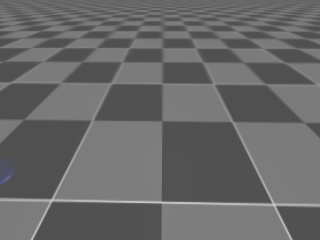
\includegraphics[width=.47\linewidth]{assets/sample_kick_front.png}\hfill
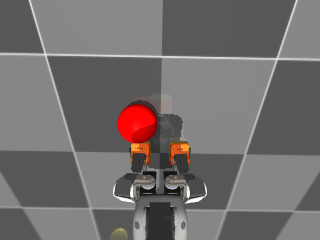
\includegraphics[width=.47\linewidth]{assets/sample_kick_near.png}
\caption{同一真实踢球样本：front 中目标红球不在视野；near 能看到脚边红球和机器人身体。前相机看不到目标，不等于两台相机都看不到。}
\end{figure}

\begin{Verbatim}[breaklines=true,fontsize=\small]
instruction = "踢红球"
state = {
  "yaw": 0.017050, "stationary": true,
  "tilt_deg": 1.392739, "sim_time_s": 0.6,
  "detections_rgbd": [{
    "color": "red", "camera": "near",
    "center_body_m": [0.090468, 0.039138, -0.080457],
    "pixel_uv": [138.0, 125.0], "pixels": 1231,
    "confidence": 0.806886, "fit_residual_m": 0.000196
  }]
}
context.previous_action = {
  "type":"skill","skill":"stand","seconds":0.6,
  "target_color":"red","reply":"保持站立，等待身体稳定。"
}
context.step = 1
context.selected_color = "red"
target = {
  "type":"skill","skill":"kick_left","seconds":0.5,
  "target_color":"red","reply":"执行左脚踢球动作。"
}
\end{Verbatim}

这份展示中的赋值写法用于讲解字段，不是可直接作为一行训练 JSON 的替代文件。context 还保存原样的 \texttt{previous\_feedback} 与一条 history：确认刚才的 stand 已执行，说明踢球任务应按新画面继续判断，执行过动作不代表踢球成功。history 的 action 与 previous\_action 相同，feedback 与 previous\_feedback 相同。以后较长任务最多保留最近六条。

这里 $z$ 为负，表示球心在躯干原点下方，并非无效深度。球心 $x,y$ 到左脚目标点的误差约为 $0.000968$\,m、$-0.001962$\,m，都小于 0.012\,m；机身也已静止。因此老师标注左脚踢 0.5\,s。该标签是规则示范，不能描述为“微调模型已经正确预测”。

原始事件观测时间约为 2.6\,s，任务首帧约为 2.0\,s，故 v5 输入时间为 0.6\,s。执行记录确认这次动作从约 2.6\,s 到 3.1\,s 完成；随后固定恢复 3\,s，再结束任务。训练只保留 stand0.6、kick0.5、finish 三次选择，恢复不是第四个需要预测的技能。

\subsection{逐字段变成模型消息}

导出行的 \texttt{images} 是数据集内双图相对路径；\texttt{instruction/state/context} 是真正输入；\texttt{target}、\texttt{label} 和 assistant 消息是同一个五字段目标。顶层 sample、episode、task、seed 及 \texttt{source} 保存追溯关系，不进入 user 文本。source 中的规则 phase、规则任务种类和真实执行时间也不是学生特征。

消息顺序固定为 system、user、assistant。system 是完整 v5 提示词；user 内容依次为“Current camera: front”、前图、“Current camera: near”、近图，最后一段 JSON 文本装入原指令、状态和历史。assistant 才放正确动作 JSON。训练器从 raw 字段重新构造同一结构，读取两张 PNG 为 RGB，交给 Qwen processor；processor 用 chat template 加上角色标记、图像占位和视觉张量。它不是只读取图片文件名就能看图。

构造 prompt 时只有 system 与 user，再加 assistant 开始标记；构造训练全文时才追加 target。程序核对前缀边界，不静默截断过长样本。模型需要预测 assistant 部分的 token，不能把 target、成功指标、未来图像混进 user，详细损失和张量处理见训练章节。

首条真实问答样本的指令是“现在能看到什么？”，老师回复“我现在看到左前方有红球，右后方有黄球。”其类型为 answer、skill 为 null、seconds 为 0。这里“视野”包括 near，所以右后方黄球可以被描述；回复没有因为场景配置固定有三球就声称看见蓝球。它证明数据里有视觉问答目标，不证明模型已具备开放世界对话能力。

\section{防止偷看答案，以及这批数据的边界}

v5 删除了模型 context 中的 \texttt{task\_id}，将绝对 episode 时间改为任务内相对秒数并舍入到微秒。原因是原连续指令顺序固定：如果“第二个任务总是前进”，模型可能根据任务编号或绝对时间猜答案。原日志仍保留编号与绝对时间方便排查；训练和部署共享同一过滤与时间函数。独立复位的六方向补充进一步提供“相同画面、不同语言、不同动作”的样本。

当前目标颜色来自原始指令；第一次决策不会得到规则已经解析好的当前 intent。执行过含颜色的动作后，历史中的 \texttt{selected\_color} 才可用于连续任务。真值只在旁路评价成功与否、筛选任务，不作为模型球心，也不会强迫模型在 finish 中声称已经成功。踢球结束标签使用“已执行踢球动作并恢复站立；是否踢中目标需要独立验收。”

\begin{longtable}{P{4.0cm}r r r}
\hline
技能标签 & 训练 & 验证 & 测试\\
\hline
\endhead
\texttt{stand} &342&60&56\\
\texttt{move\_forward} &1425&188&165\\
\texttt{move\_backward} &130&26&21\\
\texttt{move\_left} &2015&250&196\\
\texttt{move\_right} &2310&254&217\\
\texttt{turn\_left} &649&114&91\\
\texttt{turn\_right} &445&61&49\\
\texttt{kick\_left} &96&17&18\\
\texttt{kick\_right} &246&42&38\\
\hline
\end{longtable}

动作分布不均衡，横向调整明显多于后退与左踢；相邻样本也很相似，11,934 行不等于 11,934 个独立场景。随机完整踢球与已就位近场踢球必须分别评估，还要看每类技能及整任务完成情况。

老师有一个尚未完全显式化的记忆：第一次进入近区时锁定的脚别。六条动作历史不一定能恢复很久以前的决定，因而个别标签可能依赖学生未充分观测的状态。本轮已记录这一限制，没有把老师内部脚别偷偷塞给学生。以后可设计模型自己提交并保持的脚别记忆，再同步更改采集、训练和部署协议。

失败轨迹可用于诊断和以后构建纠错数据，但本轮并没有 DPO、chosen/rejected 配对或失败负样本损失。这轮 SFT 的目标是模仿经过筛选的正确技能选择，不是在训练过程中通过试错自动学会所有失败恢复。

本章数据证据：三个采集根目录的 \texttt{summary.json}、正式数据 \texttt{manifest.json}，以及独立审计 \texttt{training\_audit\_20261114/final\_dataset.json}；完整路径与关键行号列于 \texttt{sources\_local\_data.json}。

\chapter{VLM 怎样调用技能并形成闭环}
\label{chap:runtime}

这套系统把“理解画面与指令，选择下一步”和“让关节持续运动并保持平衡”放在不同层。上层输出一个技能名称及受限时长；下层用已有 ONNX 策略产生连续关节目标。训练改变的是上层选择方式，现有走路、平衡和左右踢球模型在这次微调中不更新。

\section{还没有机器人微调时，模型为什么知道技能库}

模型并不会自动扫描本机目录，也不会仅凭“你是一只小鸭子”知道有哪些动作。应用程序每次发送完整的 \texttt{SYSTEM\_PROMPT}，其中明确列出九个技能、机身坐标、方向含义、持续时间范围、两台相机的用途、脚边目标点以及回复格式。它还包含“走一步后结束”“看不见目标先转身寻找”等接口示例。这是人写的使用说明，属于推理时上下文；没有因发送提示词而更新模型权重。

预训练的指令模型已有读取图像和语言、遵循指令、生成文本的基础，因此可以尝试在这个说明下选择技能。它是否选得正确、能否持续执行完整任务，仍需测试。微调则把大量“本机画面＋原指令＋必要状态和历史 $\rightarrow$ 正确技能及参数”变成训练监督，让权重更适应这套机器人和任务。

因此至少要区分三层“已经训练”：Qwen 的通用预训练／指令训练、已有 ONNX 动作策略的训练、本次机器人技能调用的微调。代码里的 \texttt{is\_trained\_vlm=True} 只说明正在调用一个有预训练权重的模型；同处的 \texttt{robot\_finetuned=False} 明确没有加载本项目微调结果。不能把前者读成“本机微调已经完成”。

\subsection{目标颜色究竟从哪里来}

以“别踢蓝球，把红球踢出去”为例，原话直接进入 user 输入。模型需要理解要操作的是红球，再从双图和辅助检测寻找对应目标；当前技能层不调用规则解析器先替它决定红色。提示词只告诉它合法颜色值有 red、yellow、blue，没有替当前指令填写答案。

模型输出的 \texttt{target\_color} 是它本次声明的目标，不保证一定理解正确。guard 检查的是这个声明颜色的球是否可见、是否在脚边，不能代替语言理解。如果模型把红球任务说成蓝球，而蓝球又恰好符合脚边条件，仅通过 guard 也不等于完成用户任务；独立测试的 \texttt{expected\_color} 才会按预先指定的目标验收。该测试参数不送给模型。

历史 \texttt{selected\_color} 可以来自以前实际选择过的任务；用户当前明确指定另一颜色时应以新指令为准。普通前进、后退和问答的 \texttt{target\_color} 应为 null，不能因为场景里有红球就擅自生成红球任务。

\section{九个技能和五字段 JSON}

输出格式由项目的 \texttt{PROPOSAL\_SCHEMA} 与 \texttt{parse\_proposal} 定义，不是 Qwen 的天然固定输出。通用模型本来可以生成普通对话；本项目通过提示词、服务端结构约束和客户端严格解析把它限定为下表协议。

\begin{longtable}{P{3.8cm}P{6.1cm}P{4.6cm}}
\hline
字段 & 含义 & 合法值／约束\\
\hline
\endhead
\texttt{type} & 本次要执行技能、回答、澄清还是结束。 & skill、answer、clarify、finish。\\
\texttt{skill} & 要调用的已注册动作。 & 九选一；非 skill 类型必须为 null。\\
\texttt{seconds} & 本次短动作的持续时间，单位秒。 & 0.02\,s 的整数倍；非动作类型为 0。\\
\texttt{target\_color} & 此任务要操作的球颜色。 & red、yellow、blue 或 null。\\
\texttt{reply} & 面向人的简短中文说明。 & 字符串，最多 1000 字符。\\
\hline
\end{longtable}

\begin{longtable}{P{4.3cm}P{6.3cm}P{3.9cm}}
\hline
技能名称 & 底层请求 & 上层允许时长\\
\hline
\endhead
\texttt{stand} & 零速度指令，持续平衡。 & 0.02--1.00\,s\\
\texttt{move\_forward} & 前向速度指令 $+0.2$\,m/s。 & 0.02--0.60\,s\\
\texttt{move\_backward} & 前向速度指令 $-0.2$\,m/s。 & 0.02--0.60\,s\\
\texttt{move\_left} & 横向速度指令 $+0.2$\,m/s。 & 0.02--0.60\,s\\
\texttt{move\_right} & 横向速度指令 $-0.2$\,m/s。 & 0.02--0.60\,s\\
\texttt{turn\_left} & 偏航角速度指令 $+1.0$\,rad/s。 & 0.02--1.00\,s\\
\texttt{turn\_right} & 偏航角速度指令 $-1.0$\,rad/s。 & 0.02--1.00\,s\\
\texttt{kick\_left} & 调用已有左脚踢球 ONNX。 & 固定 0.50\,s\\
\texttt{kick\_right} & 调用已有右脚踢球 ONNX。 & 固定 0.50\,s\\
\hline
\end{longtable}

速度只是给行走策略的请求，短脉冲实际位移受启动、步态和动力学影响，不保证等于“速度乘时间”。技能类别是离散的，但时长还要预测，并以 20\,ms 离散化；因此比只做九分类多一个参数选择问题。本轮采用自回归 JSON 监督微调，没有另外增加九分类动作头，也没有训练 VQ-VAE 动作码本。

例如，下面是\textbf{教学假设}的格式演示，不是模型测试输出：

\begin{Verbatim}[breaklines=true,fontsize=\small]
{"type":"skill","skill":"move_left","seconds":0.20,
 "target_color":"red","reply":"向左小幅调整，再观察红球。"}
\end{Verbatim}

解析器要求恰好这五个键，不接收 Markdown 包裹、额外字段、重复键、动作列表或关节代码。它拒绝 NaN、无穷数、错误类别、非法时间和不满足 0.02\,s 步长的参数。上层 stand 最大 1\,s，而底层执行器可执行踢后 3\,s 恢复；后者是执行协议，不能由模型绕过上层约束随意指定。

本节核对：\texttt{skill\_vlm.py}:22--98、153--182；\texttt{skills.py}:14--21。

\section{一轮真实运行经过哪些部件}

\begin{enumerate}
\item \textbf{观察。} 取得当前双图和测量状态，构造 \texttt{SkillInput}，四项内容为 \texttt{instruction}、\texttt{images}、\texttt{state}、\texttt{context}。保留原话及最近六条动作／反馈；去除任务编号，使用任务内相对时间。
\item \textbf{请求模型。} \texttt{LocalVLMBackend} 把 RGB 编成 PNG，再作为图像内容发送到本机回环 HTTP 服务。消息含 system 与 user，温度为 0，最多生成 256 tokens，并请求严格 JSON schema；模型别名是 \texttt{microduck-vlm}。
\item \textbf{解析与新观测检查。} 先严格解析 JSON，再取得更新的观测做 guard。模型推理需要时间，初始图片不能直接被当作执行瞬间的状态。
\item \textbf{执行或拒绝。} guard 通过才调用 \texttt{Runtime.execute}。拒绝时不偷偷替换成规则动作，而把拒绝原因留给下一次模型决策。连续三次拒绝则结束任务。
\item \textbf{底层控制。} 对应 ONNX 读取本体状态并连续输出关节目标，MuJoCo 推进物理。记录实际开始、结束以及 completed 状态。
\item \textbf{恢复、反馈、再看。} 非站立动作自动恢复站立，普通动作 1\,s、踢球 3\,s；然后重新观察，把本次提议及实际反馈放进 history，继续同一语言任务。
\end{enumerate}

guard 对动作要求机身倾角不超过 $25^\circ$；踢球还要求身体静止、指定颜色在当前 RGB-D 测量中存在，以及球心落在对应脚目标点的双轴 $\pm0.012$\,m 区域内。它只作接受或拒绝，不替模型决定该左移还是右移。其目标也不是覆盖全部导航危险：它没有把普通移动自动变成避障规划；相关选择仍由模型负责。

上一条记录即使叫 \texttt{previous\_action}，也要结合 \texttt{previous\_feedback} 理解。部署时其中可能保存被拒绝的提议，不能因为历史里出现过 kick 就认为真的踢了；只有成功执行反馈才能证明执行。当前成功示范主要提供 \texttt{executed\_and\_recovered} 反馈，不能宣称已经充分训练了所有拒绝后的恢复行为。

推理超时、格式错误或服务异常会留下日志并结束当前任务；程序没有静默回退到规则老师。停止请求有独立通道，推理在后台线程等待时仍可取消；被取消或超时请求的迟到回复不会再进入动作执行器。

\section{50 Hz、200 Hz 和 VLM 推理不是一个频率}

MuJoCo 每 0.005\,s 走一步，执行器 controller 也在每步更新，因此是 200\,Hz。技能策略每 0.02\,s 计算一次 ONNX 输出，即 50\,Hz；随后四个物理步使用该周期的目标。模型选择一次 0.5\,s 踢球技能，意味着底层约运行 25 次 ONNX 推理、100 个物理步，不是 VLM 需要输出 100 次关节命令。

三个 ONNX 会话在 CPU 上运行：一个行走策略复用零速度、前后左右及转向命令，另两个是左右踢球。切换技能时保留上一时刻 14 维动作历史；不会每切换一次都假设机器人刚复位。导入时检查模型输入输出尺寸、关节顺序、HOME、动作缩放与模型哈希，防止同名模型接口不兼容。

\begin{longtable}{P{4.0cm}P{10.6cm}}
\hline
61 维底层输入 & 内容\\
\hline
\endhead
0--2、3--5 & 躯干角速度、躯干坐标中的单位重力方向，各 3 维。\\
6--19、20--33 & 14 个关节相对 HOME 的角度、14 个关节角速度。\\
34--47 & 上一次 14 维网络原始动作。\\
48--50 & 前向、横向和偏航速度命令；踢球调用使用零 twist。\\
51--54、55--60 & 头部 4 维、身体 6 维附加命令，本实验调用保持为零。\\
\hline
\end{longtable}

ONNX 输出形状为 \texttt{float32[1,14]}，按 \texttt{HOME + raw\_action} 得到关节目标，单位弧度，再交给执行器模型。当前仿真路径记录目标超出关节范围的幅度，未把所有目标自动裁剪成实机安全指令；不能把仿真通过等同于实体可直接执行。

VLM 则是低频、逐步决策：一次看图和生成完成，执行短动作并恢复，再请求下一次；没有固定 50\,Hz 的视觉语言推理频率。模型等待期间，实时物理线程继续执行 stand 平衡。离线规则采集不需等待大模型，可比墙钟实时更快；在线 VLM 的任务相对仿真时间会包括推理期间的站立时间。这是训练示范与部署之间仍要检验的时间分布差异。

本节核对：\path{runtime.py}:142--206、244--279；\path{skills.py}:25--92；本地 \path{microduck_deploy/policy.py}:163--222。

\section{问答、结束、澄清和停止分别做什么}

\begin{itemize}
\item \textbf{answer：} 当前任务是“看到了什么”，应根据当前图像回答，不先走路找更多东西。训练中的描述主要由规则球检测生成，语言覆盖集中在球颜色与方位。
\item \textbf{finish：} 模型报告任务已经结束。一次前进指令执行一个短脉冲并收到完成反馈后即可 finish；踢球则要继续处理搜索、接近等多个步骤。模型自述完成不等于独立物理验收成功。
\item \textbf{clarify：} 用户目标不明确时请求澄清，例如只说“踢球”却无法确定颜色。已经明确要求踢红球但红球暂时不在画面中，应先尝试寻找，不能把自己的搜索子任务推回给用户。
\item \textbf{stop：} 操作员说“停下”通过独立停止处理，不需要等待 VLM 生成一种 stop 标签；执行器取消当前脉冲并继续站立。
\end{itemize}

非动作响应均需 \texttt{skill=null, seconds=0}。没有独立目标验收时，程序对 finish 的结果标作 \texttt{model\_reported}，并提示尚未独立验收；问答为 \texttt{answered}，澄清为 \texttt{clarification}。带独立测试目标时，还会检查只发生一次有效踢球并通过整段轨迹验收，才标作 success。

默认单任务最多 40 次 VLM 调用，允许配置到 120 次；单次推理默认超时 45\,s，另有任务总墙钟 600\,s 上限。数据审计显示 457 个成功踢球示范的决策次数中位数为 21、95 分位约 56.8、最大 117，40 个超过默认 40 次。因此完整闭环评测宜显式用 \texttt{--vlm-max-steps 120}，并分别报告次数耗尽、推理超时和物理失败；最长示范距离 120 上限也只有 3 次余量。

\section{当前运行服务与正在训练的适配器}

现有 \texttt{serve\_vlm.sh} 启动的是本地 llama.cpp 服务，读取官方 Qwen3-VL-2B-Instruct GGUF：语言权重文件为 Q4\_K\_M，视觉投影相关文件为 Q8\_0。它通过回环地址提供兼容 chat-completions 的接口，不需要在每次任务时调用付费远程 API。

正在训练的 QLoRA 使用另一条 Hugging Face／Transformers 路径，保存的是适配器权重。训练目录出现 checkpoint 不会自动改变 llama.cpp 正在读取的 GGUF；当前启动代码没有自动加载这个 LoRA。后续需要明确完成合并／转换或新增兼容的推理服务，再把同一输入协议接入 \texttt{SkillTaskSession}，比较基础模型与适配器模型的同场景表现。

这一连接完成前，本报告可以证明数据和训练进程存在、训练损失在计算、模型接口与模拟执行链可用；不能把这些事实写成“微调模型已经在仿真中自动完成红黄蓝踢球”。更不能推出实体部署已经通过。本轮报告的运行范围仍是 HD1910 仿真。

\begin{notebox}{怎样理解当前系统名称}
第一阶段是预训练 VLM 驱动已有技能；微调的学习目标是视觉语言到技能及参数的映射，可按动作层级称为分层视觉语言动作策略。技术描述应同时写清：输入为双 RGB、原指令、必要状态与历史；输出为五字段技能 JSON；上层 LoRA 可训练，底层 ONNX 固定。这个描述比只争论“叫 VLM 还是 VLA”更能说明系统实际上做了什么。
\end{notebox}

本章核对：\path{skill_tasks.py}:17--37、185--315；\path{skill_vlm.py}:297--402；\path{setup_vlm.py}:30--33、280--308；\path{demo.py}:188--200。源码路径、样本来源及统计证据见同目录 \path{sources_local_data.json}。

\chapter{本次 QLoRA：一条示范怎样变成一次参数更新}

\begin{notebox}{本章描述的是正在运行的实验}
统一状态快照为北京时间 2026 年 11 月 14 日 17:14:02。正式训练已到第 101/2375 个优化步，最新完整检查点为第 100 步。这里的“已经训练”表示参数确实发生更新，不表示训练已结束，更不表示小鸭子已通过任务验收。以下参数、张量尺寸和指标以本地代码、配置与日志为依据。
\end{notebox}

\section{先确定正在训练什么}

底座是官方 \texttt{Qwen/Qwen3-VL-2B-Instruct}，固定模型版本为：
\begin{Verbatim}[breaklines=true,fontsize=\small]
89644892e4d85e24eaac8bacfd4f463576704203
\end{Verbatim}
训练读取官方 \texttt{safetensors} 权重，不读取此前用于推理的 GGUF。原始底座不被覆盖；新学到的变化保存为独立 LoRA adapter。以后使用该 adapter，仍须同时使用匹配的底座、图像处理器、提示词和技能接口。

当前做的是\textbf{监督微调（SFT）目标下的 QLoRA 参数更新}：输入真实示范中的画面、指令和允许状态，学习输出下一步技能 JSON。它不训练底层走路、平衡或踢腿控制器，也不向关节直接输出力矩。LoRA 的基本思想是在冻结权重旁增加低秩更新；QLoRA 进一步让被冻结的底座以低位宽保存，再训练这些小矩阵。\cite{lora-paper,qlora-paper}

本项目不是“所有东西都变成四位”。语言骨干中可量化的线性层使用 NF4 四位权重，并启用 double quantization；计算采用 bfloat16。视觉编码器、视觉投影与输出词表层被排除在四位替换之外。准备训练时，冻结的非量化参数中，非归一化部分转回 bfloat16，归一化部分保留 float32。视觉部分全部冻结，语言层中加入的 LoRA 参数可训练。这样的配置符合 PEFT 支持的量化底座加适配器训练路径；本地使用普通 AdamW，并没有声称启用了原论文中的全部优化手段，例如分页优化器。\cite{peft-quantization}

\begin{longtable}{@{}>{\raggedright\arraybackslash}p{3.0cm}>{\raggedright\arraybackslash}p{5.0cm}>{\raggedright\arraybackslash}p{6.8cm}@{}}
\hline
项目 & 本次设置 & 实际含义 \\
\hline
\endfirsthead
\hline 项目 & 本次设置 & 实际含义 \\ \hline
\endhead
训练参数 & 8,716,288 个 & 只统计 \texttt{requires\_grad=True} 的参数，不是模型全部参数。\\
LoRA 配置 & $r=8$，$\alpha=16$，dropout $=0.05$ & 低秩维度为 8；标准缩放 $\alpha/r=2$；训练时适配器输入使用 dropout。\\
插入位置 & 28 个语言层中的七类线性层 & 注意力的 $q,k,v,o$ 投影，以及 MLP 的 gate、up、down 投影；不在视觉层训练 adapter。\\
微批与累积 & microbatch $=1$，累积 4 次 & 同一时刻处理一条样本；累计四条的梯度后更新一次。\\
优化器 & AdamW，目标学习率 $10^{-4}$ & weight decay 为 0.01；更新前将梯度范数裁剪到 1。\\
学习率计划 & 118 步 warmup，之后 cosine & $\lfloor2375\times0.05\rfloor=118$；并非从第一步就使用最大学习率。\\
训练长度 & 1 epoch，9500 条训练样本 & $9500/4=2375$ 个优化步；\texttt{max-steps=10000} 只是上限，不会额外重复至一万步。\\
\hline
\end{longtable}

例如一个原线性映射为 $h=W_0x$。本次通过下面的形式改变行为：
\[
h=W_0x+\frac{\alpha}{r}BAx,
\qquad A\in\mathbb{R}^{r\times d_{\mathrm{in}}},\quad
B\in\mathbb{R}^{d_{\mathrm{out}}\times r}.
\]
优化器更新 $A,B$，冻结的 $W_0$ 不接收权重更新。参数变少能减少梯度和优化器状态的存储，但信息仍要穿过完整骨干。因此“只训练八百多万参数”不等于只运行一个八百万参数的小模型。

\section{一条训练样本进入模型之前}

每条样本包含 front、near 两张同一时刻的 RGB 图像、用户原始指令、允许的传感状态和历史反馈，以及教师给出的目标 JSON。RGB-D 检测结果以辅助文本状态输入；它不是第三张图，也不是直接把仿真世界的球坐标交给模型。模型可见上下文不含样本的目标答案、教师动作标签或任务编号。时间字段是当前任务开始后的相对时间。

图像处理器设置 \texttt{min\_pixels=65536}、\texttt{max\_pixels=98304}。这些数限制像素预算，不是视觉 token 数，也不是保证图像固定为某个尺寸。预处理还会按照模型的 patch 和合并因子调整图像尺寸。本次完整训练加验证数据预检得到：最短 1415 token，中位数 2356，最长 2683；系统提示词自身为 1085 token。设置的 4096 是拒绝超长输入的上限；程序没有偷偷截掉历史或任一相机。

为了将抽象过程具体化，下面列出最长训练样本经过 CPU 预处理后的真实尺寸。它的目标动作是向右移动 0.10 秒，目标颜色为蓝色。
\begin{longtable}{@{}>{\raggedright\arraybackslash}p{3.0cm}>{\raggedright\arraybackslash}p{5.0cm}>{\raggedright\arraybackslash}p{6.8cm}@{}}
\hline
张量 & 尺寸或数值 & 怎样理解 \\
\hline
\endfirsthead
\hline 张量 & 尺寸或数值 & 怎样理解 \\ \hline
\endhead
\texttt{input\_ids} & $[1,2683]$ & 一条完整聊天序列的 token 编号，含目标 JSON。\\
{\small\texttt{attention\_mask}} & $[1,2683]$ & 本例没有批内 padding；它不是“哪些 token 计入损失”的掩码。\\
\texttt{pixel\_values} & $[640,1536]$ & 两张图合计 640 个视觉 patch；每个 patch 是处理器展开后的数值，不是 640 张图片。\\
{\small\texttt{image\_grid\_thw}} & $[2,3]$，两行均为 $[1,16,20]$ & 分别记录两幅图的时间、高、宽网格；空间合并后每张图占 80 个视觉位置。\\
输入与目标边界 & 输入 2642 token，目标 41 token & 模型必须理解完整输入，但只对随后 41 个助手目标 token 计算交叉熵。\\
\hline
\end{longtable}

原始两幅 320$\times$240 图像在这一例中调整为 320$\times$256；每张有 $16\times20=320$ 个 patch，合并后为 $320/4=80$ 个视觉位置。语言隐藏维度为 2048，词表大小为 151936。这些维度说明图像和文字最终如何共同进入语言骨干；它们不代表额外增加了一台相机。

当前 \texttt{encode()} 为了严格核对助手边界，对“完整序列”和“只有输入的序列”分别调用一次 processor。因此 CPU 图像预处理与分词会重复；这不等于在同一次训练前向中把视觉编码器运行两遍。冻结视觉特征目前也没有离线缓存，每条样本仍会经过视觉前向。

\section{为什么训练时把正确答案也放进输入}

这是自回归监督训练的 teacher forcing。假设目标 JSON 被分词为 $y_1,y_2,\ldots,y_T$，训练时同时提供完整序列，但通过因果注意力约束，预测 $y_t$ 时只能看到原始输入和 $y_1,\ldots,y_{t-1}$，不能看到当前位置和未来的正确 token。

例如模型预测 \texttt{move\_right} 时，允许使用前面已经给定的 JSON 键名；它不能直接读取正在预测的答案。对第一枚助手 token，则使用输入末尾位置产生的 logits。推理时没有正确答案可供拼接，模型要逐个使用自己已生成的 token，因此训练损失下降与自由生成正确率并不等价。

本地实现采用显式因果移位。设输入长度为 $P$，完整长度为 $L$，取预测位置 $P-1$ 至 $L-2$，对应标签位置 $P$ 至 $L-1$。本例 $P=2642,L=2683$，所以预测位置为 2641 至 2681，标签位置为 2642 至 2682，共 41 个。

\texttt{logits\_to\_keep} 只要求词表输出层计算这些位置，得到约 $[1,41,151936]$ 的 logits。它\textbf{没有删掉前面 2642 个输入 token 的注意力上下文}。若在所有位置都构建词表 logits，中间张量会大得多；这是本次能在小显存上运行的一个关键实现选择。

每条样本的损失是：
\[
\ell_i=-\frac{1}{T_i}\sum_{t=1}^{T_i}
\log p_\theta(y_{i,t}\mid x_i,y_{i,<t}).
\]
这里 $x_i$ 包括图像、指令和状态；$T_i$ 是该样本被监督的助手 token 数，包括 JSON 内容及相应结束 token。输入提示词自身不直接计入交叉熵，\texttt{reply} 文本和 JSON 标点却会计入，所以低 loss 可能部分来自学会固定格式。它不是“踢球距离的误差”，也没有直接奖励球被踢远。

该 selected-logits 实现曾用小型模型在 CPU 上对照标准 masked-label loss：损失差约 $4.77\times10^{-7}$，梯度最大差约 $5.96\times10^{-8}$；另检查了改变未来标签不影响更早预测。它验证损失实现的对应关系，不验证机器人能力。

\section{四条样本怎样合成一次更新}

程序依次处理四条样本，每条执行 \texttt{(loss / 4).backward()}，梯度累加在同一套 LoRA 参数上。四次反向传播完成后，才执行梯度裁剪、AdamW 更新、学习率调度，并清空梯度。
\[
\mathcal{L}=\frac{\ell_1+\ell_2+\ell_3+\ell_4}{4},
\qquad g=\frac{1}{4}\sum_{i=1}^{4}\nabla_\theta\ell_i.
\]
日志中的 \texttt{train\_loss} 也是这四个样本损失的平均。每条先做 token 平均，因此不同长度的样本仍然等权；它不等于将四条的全部 token 混在一起后统一平均。若最后只剩不足四条，程序使用实际剩余条数归一化。本次 9500 能被 4 整除，没有最后一个不完整批次。

“有效 batch 为 4”说的是更新所汇总的样本量。当前只有一个训练进程、一块 GPU，微批大小为 1；不是四个样本并行，也不是四块 GPU。CPU 的六个计算线程不改变这个事实。GPU 内部仍会并行处理矩阵和同一序列中的位置。

\section{验证、保存与恢复分别证明什么}

训练前，对固定 32 条验证样本计算 teacher-forced loss；之后每 100 个优化步及末步重复验证。另在训练前和全部训练完成后，各对固定 24 条验证样本进行自由生成，最长新增 192 token，不强制 JSON 语法。这 24 条按照九种技能和 answer、clarify、finish 共 12 类轮流抽取，每类两条；它不是完整 1299 条验证集，更不是 1135 条测试集。

初始量化底座的结果如下。分母统一为全部 24 条，解析失败也算错；并不是只在合法 JSON 中计算准确率。
\begin{longtable}{@{}>{\raggedright\arraybackslash}p{5.0cm}>{\raggedright\arraybackslash}p{3.0cm}>{\raggedright\arraybackslash}p{6.8cm}@{}}
\hline 指标 & 初始结果 & 需要注意 \\
\hline
JSON 合法 & $20/24=83.3\%$ & 满足解析器与字段约束，不表示动作正确。\\
type 正确 & $18/24=75.0\%$ & 区分动作、回答、澄清和结束。\\
skill 正确 & $7/24=29.2\%$ & 分母含非动作样本的 null，不能直接称为九技能准确率。\\
颜色正确 & $17/24=70.8\%$ & 包括 null；仍需另看红黄蓝各类。\\
时长精确一致 & $9/24=37.5\%$ & 包括非动作的零时长；数值近似但不相同也算错。\\
四字段联合正确 & $6/24=25.0\%$ & 同时比较 type、skill、颜色和时长；不评价 reply 语义。\\
\hline
\end{longtable}

固定 32 条验证样本的平均 loss 从初始 1.01327 降到第 100 步的 0.16867，这是快照中已观察到的进展。第 100 步没有运行新的 24 条自由生成；因此不能据此写出“微调后联合正确率”。更不能从单步标签匹配推出转身搜索、靠近、对齐、踢球的整段任务成功率。

检查点在第 10 步、之后每 50 步和最终步保存。每个完整检查点含 adapter、优化器状态、调度器状态、CPU/CUDA/Python 随机数状态、数据游标和配置指纹。目录先写入唯一临时位置，再原子发布；只保留最近两个完整检查点。\texttt{best\_adapter} 按验证 loss 单独保留，最终 adapter 在正常结束时保存。

恢复会核对数据、提示词、学习率、累积数、训练长度等参数，并从确定的数据顺序和已保存游标继续。若中断发生在两次保存之间，那部分更新需重算；SIGINT 不会把半个累积批次冒充完整检查点。恢复能力也不等于保证所有 CUDA 运算逐比特相同。

\section{这台电脑为什么约需十几个小时}

已测约 22 秒完成四条样本的一次更新，即约 5.5 秒/样本。9500 条的纯训练估计约 14.6 小时，加上验证和生成，首轮估计 15--17 小时；这是当时吞吐的估算，不是完成时间承诺。主要明确存在的工作量包括完整骨干计算、双图视觉前向、长上下文注意力、量化运算，以及为节省激活显存而进行的 gradient checkpointing 重算。

本次正式运行已观察到 PyTorch 峰值 allocated 约 3409.9 MiB、reserved 4318 MiB，整卡占用约 5300 MiB（5.2 GiB）。allocated 是活跃张量使用量，reserved 还包含 PyTorch 缓存池，整卡统计另含 CUDA 上下文、桌面显示和其他驱动开销。不能用整卡占用直接推算“模型权重有多大”，也不能把空闲显存与模型文件大小直接比较。

GPU 高利用率支持“GPU 端持续忙碌”的判断，但没有详细 profiler，就不能给算力、显存带宽和 CPU 处理分别标出准确百分比。四位权重也不保证四倍加速；增加累积次数不会让每条样本少做前后向。更大微批能否装下、更换注意力实现能快多少，都尚未做对照实测。此前资源测试只证明双图、最长上下文和优化器能在 6 GB 机器上运行；它不替代任务评估。

\section{本地证据在哪里}

以下路径均相对于 \texttt{/home/luckysir/Strands\_Robots}。训练仍在继续，实时文件会更新，文档状态以本章开头的快照为准。
\begin{Verbatim}[breaklines=true,fontsize=\small]
experiments/microduck_tasks/train_vlm.py
experiments/microduck_tasks/setup_training.py
experiments/microduck_tasks/launch_training.py
experiments/microduck_tasks/training_requirements.txt
.cache/microduck_train/model/
experiments/microduck_tasks/outputs/training_dataset_final_20261114/
experiments/microduck_tasks/outputs/qlora_20261114/training_config.json
experiments/microduck_tasks/outputs/qlora_20261114/preflight.json
experiments/microduck_tasks/outputs/qlora_20261114/metrics.jsonl
experiments/microduck_tasks/outputs/qlora_20261114/baseline_evaluation.json
experiments/microduck_tasks/outputs/qlora_20261114/latest_checkpoint.json
experiments/microduck_tasks/outputs/qlora_20261114/startup_verification.json
experiments/microduck_tasks/outputs/resource_verification_20261114/
  resource_verification.json
\end{Verbatim}

\chapter{微调方案怎样选：训练目标与更新参数是两回事}

\section{先分清两个维度}

“用什么误差教模型”和“允许哪些参数改变”是两个独立选择。SFT、偏好学习、强化学习描述学习目标和反馈形式；训练分类头、LoRA、QLoRA、局部解冻、全量更新描述参数与存储方式。不能把它们排成互相替代的一列。例如当前方案同时属于 SFT 和 QLoRA；DPO 也可以只更新 LoRA，而不必更新全部底座。

另一条独立维度是输出形式：可以生成 JSON 文本，可以直接输出技能分类概率，也可以预测连续动作。它们不由“使用 VLM”这三个字自动决定。小鸭子已有可靠的底层技能时，首先要学的是\textbf{根据观察选择技能、参数和结束时机}；是否训练关节控制器是另一项工作。

\begin{longtable}{@{}>{\raggedright\arraybackslash}p{2.0cm}>{\raggedright\arraybackslash}p{3.0cm}>{\raggedright\arraybackslash}p{5.0cm}>{\raggedright\arraybackslash}p{4.5cm}@{}}
\hline 方式 & 更新什么 & 输入、输出与数据 & 成本与能力边界 \\
\hline
\endfirsthead
\hline 方式 & 更新什么 & 输入、输出与数据 & 成本与能力边界 \\ \hline
\endhead
仅提示词 & 无参数更新 & 图像、指令、状态进入原模型；提示其生成技能 JSON；可放少量示例。 & 无训练成本但仍有推理成本；接口描述会进入上下文，不能保证遵从。\\
冻结骨干加头 & 新增 linear 或 MLP 头 & 先获得联合图文状态特征，再监督技能及参数；输入需有正确标签。 & 头很小，特征可缓存；适应能力受冻结特征限制，任意文本回复还需额外路径。\\
局部解冻 & 投影器或选定后层 & 可用 JSON 示范或分类标签，目标与输出由设计决定。 & 比全量少更新，但仍有前后向开销；要防止破坏原有对齐。\\
LoRA & 各层少量低秩矩阵 & 可用于文本 SFT，也可与动作头联合训练。 & 优化器存储较小，骨干通常仍占较多显存；能力需实测。\\
QLoRA & 量化冻结底座旁的 LoRA & 当前为双图、指令、状态到下一步 JSON。 & 已验证本机可运行；量化减少存储，并非免除骨干计算。\\
全量 SFT & 所选模型全部参数 & 通常需较多且多样的高质量示范；输出仍可选择。 & 梯度、优化器和激活需求大，6 GB 本机未验证；易过拟合或遗忘。\\
DPO 等偏好学习 & 可用 LoRA 或全量更新 & 同一输入配更好和更差的输出，学习相对偏好。 & 需要可信偏好对；不是已有单一正确标签直接换个开关。\\
环境强化学习 & 上层策略或底层控制器 & 状态、动作、轨迹、奖励和终止信号；目标是累计回报。 & 需要大量交互与奖励设计；能优化长期任务，但训练复杂度更高。\\
\hline
\end{longtable}

表中只有“提示词驱动现有技能”和“当前 JSON QLoRA 训练链路”已经在本项目中实现。分类头、投影器微调、全量 SFT、DPO 与上层强化学习均是可研究方案，不是已经配置好的启动命令。它们的准确率和训练时间不能从当前 QLoRA 日志推算。

\section{方案一：冻结 VLM，只训练技能预测头}

这通常是一个很值得做的对照实验。先让冻结的 VLM 将允许输入变成向量，再让一个小网络学习如何将这个向量映射到技能。冻结特征后训练新层、或预先保存特征再训练小模型，是标准迁移学习流程；官方 Keras 指南也明确说明了缓存能减少重复骨干计算，以及动态数据增强会使固定缓存不再适用。\cite{transfer-feature-cache}

\subsection{必须缓存联合输入特征，不能偷看目标}

对于第 $i$ 条样本，先构造：
\[
z_i=F_{\theta_0}(I_i^{\mathrm{front}},I_i^{\mathrm{near}},
u_i,s_i,h_i),\qquad \theta_0\ \text{保持冻结}.
\]
这里 $u_i$ 为用户指令，$s_i$ 为允许状态，$h_i$ 为历史。对于因果 VLM，一种候选读出位置是\textbf{助手开始标记之前或完整输入末端的隐藏状态}，它已能注意到前面的图像、指令和状态；也可以比较输入位置池化。究竟哪种读出更适合技能预测需要验证，不应把“最后一个向量”当成已证明的最佳表示。

缓存时绝不能将目标 JSON 接在后面，再从回答末端取向量。那样特征已经读到了正确技能，训练和离线测试可能看起来极好，上线时却拿不到这样的特征。教师动作、规则阶段、仿真世界坐标、任务编号、文件名中的标签也不能偷偷混进输入。相同画面配“踢红球”和“踢蓝球”时，联合特征应允许因指令不同而不同；只缓存图像向量后直接分类，会丢掉语言条件。

缓存还应固定底座版本、提示词、处理器、取特征位置和推理模式，并为缓存记录输入与配置哈希。图像或文字增强改变了输入，就应重新提取对应特征；一旦开始更新骨干或 LoRA，旧联合特征也会失效。数据的 train、val、test 划分必须在特征训练前固定，标准化统计只从训练部分估计。

若每条只保存一个 2048 维 float16 向量，9500 条训练样本的数值本体约为 $9500\times2048\times2$ 字节，即 37.1 MiB，另有标签和元数据。这是\textbf{所提缓存格式的体积估算}，不是已经产出的文件。离线提取仍须为每条运行一次 VLM；实时机器人每获得新画面，也仍要运行一次骨干。缓存主要加快反复训练小头，不能把未来从未见过的画面提前算好。

\subsection{四个头分别预测什么}

可以在共享特征上建立一个 linear 头，或先接小型 MLP，再输出四组 logits：
\[
(a^{\mathrm{type}},a^{\mathrm{skill}},a^{\mathrm{duration}},a^{\mathrm{color}})
=H_\phi(z).
\]
一个与当前接口对应的候选设计如下。
\begin{longtable}{@{}>{\raggedright\arraybackslash}p{3.0cm}>{\raggedright\arraybackslash}p{5.0cm}>{\raggedright\arraybackslash}p{6.8cm}@{}}
\hline 预测头 & 类别 & 使用方法 \\
\hline
type & 4 类 & skill、answer、clarify、finish，所有样本监督。\\
skill & 9 类 & stand、前后左右移动、左右转向、左右踢；仅动作样本计算该项损失。非动作输出 null。\\
duration & 51 个候选格点 & $0,0.02,\ldots,1.00$ 秒；根据 type 和 skill 屏蔽不合法值。\\
color & 4 类 & red、yellow、blue、null；所有样本可监督，学习无颜色目标的情况。\\
\hline
\end{longtable}

这个设计不能随意把任何头的最大概率组合起来。例如非动作必须 \texttt{skill=null, seconds=0}；移动时长只能为 0.02 至 0.60 秒，站立和转向为 0.02 至 1.00 秒；两种踢球固定 0.50 秒。可以先选择 type，再在对应合法技能与时长集合中解码。训练 duration 项也使用正确技能对应的合法集合，推理则必须使用预测技能，不能继续用真值来替模型纠错。

颜色不能简单规定“非动作一律 null”。本地示范中，完成踢红球任务的 finish 仍可保留 red；而回答视野问题通常为 null。哪些结构组合不合法可由接口确定，但“这次应该选蓝色还是红色”是需要学习的内容，不能用测试标签建立屏蔽表。

一种起点损失为：
\begin{align*}
\mathcal{L}_{\mathrm{head}}={}&
\lambda_t\operatorname{CE}(a^{\mathrm{type}},t)
+m_s\lambda_s\operatorname{CE}(a^{\mathrm{skill}},k)\\
&+m_d\lambda_d\operatorname{CE}(a^{\mathrm{duration}},d)
+\lambda_c\operatorname{CE}(a^{\mathrm{color}},c).
\end{align*}
其中 $m_s$ 只在 type 为 skill 时取 1；$m_d$ 只在需要学习可变时长的动作上取 1。固定踢球时长可直接由接口赋值，避免训练一个没有选择余地的分类项。各权重可先设为 1，再依据验证集调整，不能为了提高测试分数反复改测试配置。若少数技能严重不足，可以在训练集内采用类别权重或分层采样，同时保持评估分布清楚可追溯。

例如“向前一点”的正确标签可以为 skill、move\_forward、0.32、null。若模型把类型判成 finish，即使另一个头恰好选对 move\_forward，最后动作仍然错。评估必须查看联合结果，而不只是分别挑最好看的单头准确率。分类概率也不天然是可信置信度；若使用低置信度转为 clarify，需要在验证集上校准并检查是否滥用澄清来逃避任务。

\subsection{技能头怎样保留“你看到了什么”}

分类头只输出有限类别和参数，不能凭空生成自由中文 \texttt{reply}。一种完整部署方案是：动作、结束和固定澄清由头决定并填充模板；当 type 为 answer 时，再调用冻结 VLM 的文本生成能力回答当前画面。另一种方案是另训练回复解码路径，但那已超出“只训练小分类头”。

因此比较两种方案时，应分别测动作决策和视觉问答。不能把只会输出 skill ID 的小头称为已经拥有完整对话功能，也不能假定冻结底座的回答在新的仿真视角上一定正确。无论哪种输出方式，最终都要转换为同一个技能协议，再经过相同的时长约束、踢球条件和执行反馈闭环。

\section{其他参数更新方法何时有意义}

\subsection{投影器或局部解冻}

当图像特征对新相机外观、视角或任务细节不够适配时，可以研究更新视觉到语言的投影模块、语言末端若干层，或小部分视觉层。它比全冻结有更多调整空间，但“解冻一小块”并不自动意味着显存很小：只要梯度要穿过相关路径，就需要保存或重算激活。当前视觉编码器和投影器全部冻结，尚无这一方案的本机性能结论。

应先检查错误来自哪里。若颜色识别已对，错误集中在何时停止，先改善上层示范和时序监督通常比改视觉模块更直接。若目标在图中只有几个像素，换训练参数也未必能弥补输入分辨率缺失；需要一起评估图像设置、相机覆盖和数据质量。

\subsection{LoRA、QLoRA 与全量 SFT}

LoRA 用低秩矩阵表达权重变化，QLoRA 则把它与量化冻结底座结合。选择 $r$ 是容量与成本的权衡，不是准确率旋钮；更大 $r$ 需要更多可训练参数，也可能更容易记住有限示范。本次 $r=8$ 是经过显存验证的起点，不代表已经搜索过全部最优配置。\cite{lora-paper,qlora-paper}

全量 SFT 允许原模型大量参数直接更新，适应空间更大，但也需要存放更多梯度与优化器状态，且可能损伤原有视觉语言能力。“全量微调”仍然从预训练权重出发，和随机初始化后从零训练不同。现有 6 GB 环境没有验证全量方案；不能直接套用当前 QLoRA 的 15--17 小时估算。

如果冻结特征小头明显欠拟合、数据质量可靠，再考虑增大头、训练部分适配器或局部解冻，可以更清楚地识别新增复杂度是否有效。每改变一次可训练范围，都应单独记录数据、参数量、资源和评测结果，而不是同时改变所有设置后把改进归因于某一个名词。

\section{偏好学习和强化学习不是“更高级的微调按钮”}

DPO 使用同一输入下的偏好输出对，促使模型提高更好输出相对于更差输出的倾向。它需要明确的 chosen/rejected 数据，方法本身不等于让机器人在线探索。原论文将其作为不必显式训练奖励模型的偏好优化方式。\cite{dpo-paper}

对小鸭子，可以研究“目标偏左时，小幅左转”优于“直接踢球”的偏好，但不能仅因某个输出来自现有规则就自动认为它永远更好。有效偏好应结合执行结果、对齐程度和任务完成情况。当前数据主要是输入到单一教师动作，尚没有经过验证的偏好对或 DPO 训练代码。

强化学习则让策略通过环境交互，优化整个轨迹的累计奖励，例如正确球被踢动的奖励、错误球接触的惩罚、跌倒或超时惩罚。奖励和终止条件定义不好，策略可能找到“看起来得分但任务没完成”的行为。语言模型领域的 RLHF 展示了示范、偏好与后续强化优化可以组合，但这不直接证明同一流程能迁移到本机器人。\cite{instructgpt-paper}

还需区分层级：训练上层“选择左转还是踢球”的策略，可以继续复用底层控制器；训练底层步态或踢腿，是另一套状态、动作频率和奖励。本次上层 QLoRA 只模仿示范，没有在线奖励优化，也不会在每次日常执行动作后自动再训练一轮。

\section{怎样公平比较小头与当前 JSON 方案}

比较应使用相同的训练、验证、测试划分和独立场景种子，输入相同两幅图、同一指令及允许状态，采用同样的技能库与执行器。两种方法可以选不同输出表示，但不能给一方额外的目标坐标或未来反馈。任何特征缓存都只能由该条允许输入产生。

离线部分至少报告合法输出比例、动作样本上的九技能准确率和混淆矩阵、每种颜色准确率、时长误差与精确一致率、四字段联合准确率，以及视觉回答是否符合图像。分类头天然容易保证结构合法，JSON 模型需要生成正确结构；应分别报告原始输出质量和进入同一执行 guard 后的结果，避免比较口径不一致。

闭环部分使用相同新场景和任务说法，测正确颜色球的实际踢动成功率、错误球动作、搜索步数、耗时、失败与拒绝原因。还应测试目标最初在盲区、靠近时暂时出视野、执行被拒绝后的调整，以及“往前一点”完成后能否停止。离线标签存在多种合理解时，精确匹配低不一定说明任务差；反过来，离线匹配高也可能在连续执行中积累误差。

成本比较要包括特征提取时间、后续训练时间、峰值显存、实时每次决策延迟和总实验迭代成本。缓存方案不能只报小头训练几秒而省略首次 VLM 提取；当前 JSON 方案也不能只报权重小而忽略逐 token 生成时间。测试集用于最终报告，不用于反复选择头大小、阈值或提示词。

截至本报告快照，已经具备的是可恢复的 QLoRA 训练、独立数据划分和初始离线基线。冻结联合特征加多头分类器是一项清晰、可复用现有数据的后续对照方案；其收益必须通过上述共同标准验证，不能先把它写成更快且更准的既定结论。

\chapter{如何知道训练有效：从损失到完整任务}
\section{训练损失正在下降，究竟学到了什么}
训练目标是让目标JSON中的token获得更高概率。开始时，模型可能在字段名称、格式、中文回复、动作名称或时长上与示范不同。只要这些差异减少，损失就可能下降。因此，损失下降是学习信号，但它把多种能力混合在一起，不能单凭一个数字判断踢球是否更准确。

例如，“回复更接近示范措辞”“更稳定输出五个字段”“选对了踢球脚”都会改变损失。前两项改善可能很快，第三项仍需要基于任务的独立检查。相邻步损失也会因抽到的四条样本难度不同而上下波动，不能把某一步低损失当成所有场景都已经学会。

\begin{figure}[htbp]
\centering
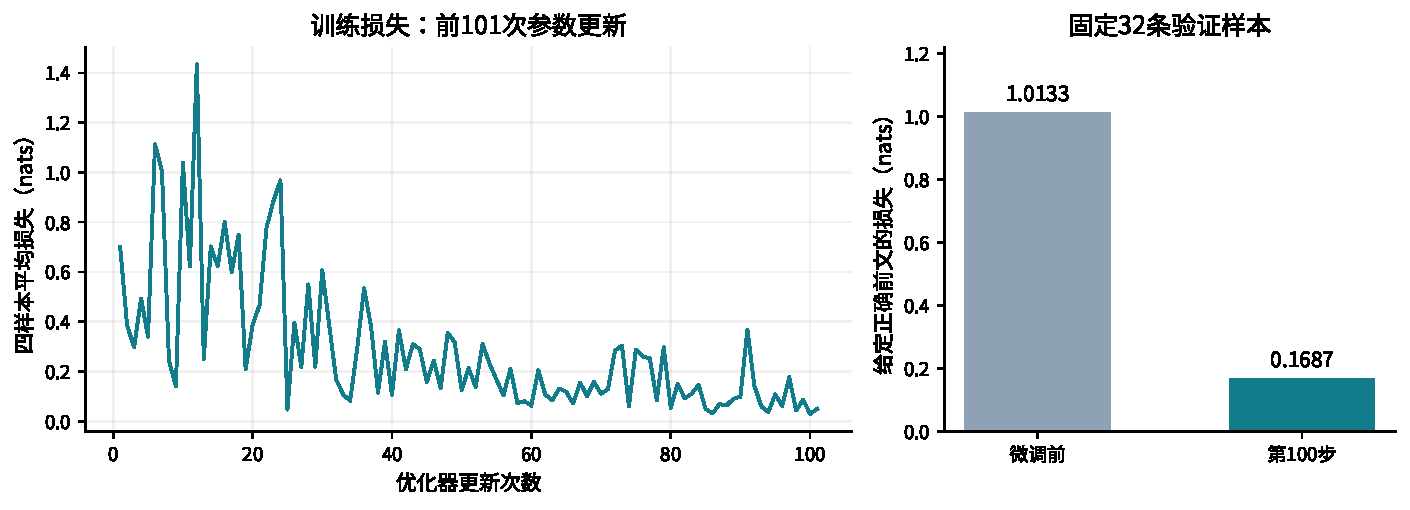
\includegraphics[width=\linewidth]{assets/training_snapshot.pdf}
\caption{真实日志快照：前101步训练损失，以及固定32条验证样本的teacher-forced损失。两个面板对应不同数据，不能直接互换解释；本图不包含微调后闭环成功率。}
\end{figure}

本书冻结的快照显示：训练前，32条固定验证样本的平均损失为1.013274；第100次更新时为0.168665。图中的nats表示使用自然对数计算的损失单位。这个下降说明模型更倾向于输出这些已知验证示范中的目标token。验证集没有参与反向更新，但反复查看同一小子集仍可能影响选模，最终必须在独立任务上验证。

\section{第一级：代码、数值与数据一致性}
首先检查程序有没有正确训练：输入长度是否超限；图片是否与样本对应；模型是否只更新指定参数；梯度是否有限；优化器步数与数据游标是否一致；保存和恢复后是否从正确位置继续；数据文件和基础模型的哈希是否符合固定清单。

当前流程已经做过短训练资源验证、恢复检查，以及正式第10步适配器与优化器状态核验。LoRA-B参数出现实际非零更新，说明训练不是只打印日志。它仍属于实现与资源证据，不是学习效果验收。

\section{第二级：给定画面时，模型自己生成什么}
训练期间的teacher forcing会给模型提供此前的正确目标token；真正生成时，后续内容依赖模型自己刚生成的token。一次早期格式错误可能影响整个JSON，所以必须单独做无强制答案的生成测试。

当前 \texttt{predict\_examples()} 会删除输入中的助手目标，只保留生成起点之前的内容，采用贪心生成，最多生成192个新token，然后把原始输出交给同一严格JSON解析器。原始输出和解析错误都写入 \texttt{predictions.jsonl}，没有偷偷修正成正确动作。

\begin{longtable}{P{33mm}P{58mm}P{60mm}}
\toprule
指标 & 当前定义 & 解释边界\\
\midrule
\endhead
JSON合法率 & 被严格解析器完整接受的输出数 / 全部样本数 & 仅合法不代表动作合适\\
type准确率 & action type与目标一致的样本数 / 全部样本数 & 区分skill、answer、clarify、finish\\
skill准确率 & skill字段与目标一致 / 全部样本数 & 包括非动作样本中null的匹配，不等于纯动作分类准确率\\
颜色准确率 & target\_color字段完全匹配 / 全部样本数 & 无颜色任务的null也计入\\
时长准确率 & seconds字段数值完全匹配 / 全部样本数 & 合理但不同的时长仍可能算错\\
联合准确率 & 上面四个字段同时匹配 / 全部样本数 & 不校验reply语义，不代表物理成功\\
分类型统计 & 每个skill或回复类型的样本数、合法数、联合正确数 & 目前小子集每类样本很少，波动较大\\
\bottomrule
\end{longtable}

解析失败样本在准确率分母中保留，并记为不正确。这样可以避免“只看解析成功的那部分”人为抬高准确率。另一方面，\texttt{reply}的描述是否忠实于图像，仍需要单独评价；不能因为四个结构字段一致就认为自由问答完全正确。

\section{当前确实存在的基线结果}
固定24条分层验证样本在未微调基础模型上的结果如下。该小集合按技能与回复类型抽样，用来作快速对照，并不是全量验证集的比例估计。

\begin{center}
\begin{tabular}{lr}
\toprule
未微调基线指标 & 结果\\
\midrule
JSON合法率 & 20/24 = 83.3\%\\
type准确率 & 75.0\%\\
skill准确率（含null） & 29.2\%\\
颜色准确率（含null） & 70.8\%\\
时长准确率 & 37.5\%\\
四字段联合准确率 & 6/24 = 25.0\%\\
\bottomrule
\end{tabular}
\end{center}

截至本书快照，正式训练后尚未完成这一组生成指标与闭环测试。早期资源试跑使用过不同版本提示词，其结果不能混入这次v5正式实验。第100步的验证损失改善也不能替代尚未完成的生成测试。

\section{第三级：在仿真中从头完成任务}
离线评测给模型的是规则老师轨迹上的观测。部署时，模型自己的选择会改变下一幅画面：少走一点、多转一点、提前踢一下，都会产生训练中较少见的状态。这种输入分布变化，是行为克隆需要闭环验证的主要原因。

完整踢球验收应从新的初始状态开始，给出明确颜色指令，允许模型搜索、靠近、对齐、踢球，最后由独立程序读取真实接触和位移证据。需要同时报告：
\begin{enumerate}
\item 目标是否找到，是否在看不到目标时错误声称目标不存在。
\item 是否到达可踢位置，是否重复动作、来回振荡或过早结束。
\item 是否选择正确颜色、正确脚，是否碰到非目标球。
\item 踢前是否提前推球，踢球是否产生目标脚接触与足够位移。
\item 是否恢复站稳，有无摔倒、超时、拒绝或决策次数耗尽。
\item 总模型调用次数、每次推理耗时、总墙钟时间和仿真时间。
\end{enumerate}

近脚已对准任务和随机远距离任务必须分开。前者只需较少动作，后者包含搜索和长期控制。把两类混合后得到较高成功率，可能掩盖导航能力不足。

当前默认VLM上限是40次决策；采集的合格踢球示范中，有40个任务需要超过40次决策，最长117次。因此后续闭环对照应显式设为 \texttt{--vlm-max-steps 120}，并独立记录每任务600秒墙钟上限。调整上限只保证任务有足够机会执行，不保证它会成功。

\section{怎样公平比较QLoRA与“方案一”}
\begin{enumerate}
\item 保持训练、验证、测试种子划分相同，按验证集选择设置，最后才使用测试集报告成绩。
\item 两种模型获得相同两路图像、语言、姿态、RGB-D辅助测量与历史长度。若一方没有深度辅助，应单独列为另一实验。
\item 保持相同技能库、执行器恢复时间、guard条件、每任务决策和墙钟上限。
\item 分别统计九个技能、三种颜色、盲区搜索、近脚踢球和直接运动，而不只看总体平均。
\item 报告显存、首轮特征提取成本、训练时间、在线决策延迟和成功率。冻结头缓存后的训练速度不能直接当成整套部署速度。
\item 从原始预训练VLM提特征的方案，与从QLoRA适配后的VLM提特征的方案应分开命名；后者已经利用了前一轮训练。
\end{enumerate}

\section{失败数据什么时候能够帮助学习}
当前保留了23个失败踢球任务的原始记录，但没有把它们作为正确动作监督。仅保存“失败了”的标签，不会自动告诉模型哪一步应该改成什么动作。

下一轮有三种不同处理方式。第一种是人工或可靠老师为失败状态补上正确的下一步动作，形成新的SFT样本；第二种是构造同一输入下经过核验的较好和较差输出，用于偏好学习；第三种是在可控仿真中定义奖励并训练策略。三者需要不同数据与训练目标，不能把失败轨迹直接混入当前成功示范JSON损失中。

对于这个项目，补充模型实际走偏后的状态尤其有价值。比如“红球仍在左侧，刚才右转错误，下一步应当左转纠正”需要真实观测、允许的执行历史和经过验证的纠正动作。纠正动作不能只根据最终失败倒推猜测，也不应把后续才知道的真实结果放回当前输入。

\section{完成这一轮之后，怎样决定下一步}
先检查生成输出是否稳定合法、运动命令是否能执行一次后结束，再评估近脚踢球，最后评估盲区搜索与随机远距离踢球。如果格式很好而搜索差，优先检查搜索数据与历史表示；如果目标颜色常错，检查同一画面不同语言目标的数据覆盖；如果对齐时来回摆动，检查距离特征、动作时长分布及规则老师隐藏锁脚状态。

还应单独检查视野问答。当前监督主要描述球，不应把模型答出某些新物体名称视为已验证能力。开放问答需要新的场景、多样物体及明确评价准则。模型训练完成这个文件状态，只表示优化流程到达计划终点；是否适合接入日常交互，要由这些具体评测决定。

\chapter{本机操作手册：查看、评测、续训与部署}
\section{先找到主要目录}
以下路径以项目根目录 \texttt{/home/luckysir/Strands\_Robots} 为起点。阅读PDF中的命令并不会执行它们；“暂停”“续训”“采集”一类命令会改变运行状态，应按你的实际目的选择执行。

\begin{longtable}{P{46mm}P{105mm}}
\toprule
用途 & 位置与说明\\
\midrule
\endhead
训练环境 & \path{.cache/microduck_train/venv}；通过只读路径复用已有Torch/CUDA，其余训练依赖在独立环境中安装\\
基础训练权重 & \path{.cache/microduck_train/model}；固定官方原始权重，用于NF4加载和LoRA训练\\
正式数据 & \path{experiments/microduck_tasks/outputs/training_dataset_final_20261114}；训练过程中不追加或改写\\
正式训练产物 & \path{experiments/microduck_tasks/outputs/qlora_20261114}；日志、状态、适配器与检查点\\
原有GGUF推理服务 & \path{.cache/microduck_vlm}；与QLoRA训练权重及输出分开\\
\bottomrule
\end{longtable}

不要删除被训练环境通过路径复用的 \path{/home/luckysir/microduck/microduck_rl/.venv}。训练环境目录较小，不代表全部运行库都位于这个目录。源码、模型、环境、缓存和数据承担不同角色，不能仅按名称中带“cache”判断是否可以随时删除。

\section{查看日志与实时状态}
\begin{Verbatim}
cd /home/luckysir/Strands_Robots
tail -f experiments/microduck_tasks/outputs/qlora_20261114/train.log
\end{Verbatim}
按 \texttt{Ctrl+C} 退出的是日志查看。后台训练由另一个进程运行，关闭这个终端不等于停止训练。电脑仍需要保持开机、不休眠。

另一个终端可以读取结构化状态：
\begin{Verbatim}
cd /home/luckysir/Strands_Robots
python3 -m json.tool \
  experiments/microduck_tasks/outputs/qlora_20261114/run_status.json
nvidia-smi
\end{Verbatim}
\texttt{step}是优化更新次数，\texttt{micro\_cursor}是已处理样本游标。本轮正常情况下 \texttt{micro\_cursor = step * 4}。训练状态文件只在特定阶段或每次更新后写入；短时间没有变化不等于进程卡死。初始全量输入预检和生成评估可能较长。

查看最近可恢复检查点时，读取指针而不是长期记住某一个编号：
\begin{Verbatim}
cat experiments/microduck_tasks/outputs/qlora_20261114/latest_checkpoint.json
\end{Verbatim}
系统只保留最近两个完整检查点，所以第10步目录在后续训练中可能被正常清理；本书中“已验证第10步”描述的是历史验证事件。

\section{中途测试：当前已实现的是离线评测}
本机6GB显卡在训练期间余量很小。现有 \texttt{--eval-only} 也会加载模型到GPU，因此应先让训练进程退出并释放显存，评测结束后再恢复。进程的 \texttt{SIGSTOP} 只是挂起，会保留显存，不能达到这个目的。

下面是“明确选择现在测试时”使用的流程。它不会把未完成的梯度累计保存为完整更新。最新检查点之后尚未保存的更新，会在续训时重新计算。

\subsection{第一步：确认有检查点，再停止对应训练进程}
以下Python块检查运行身份后发出SIGINT，不使用宽泛的进程名批量结束程序。命令会等待目标进程退出；若提示还没有检查点，继续训练并稍后再试。

\begin{Verbatim}
cd /home/luckysir/Strands_Robots
python3 - <<'PY'
import json, os, pathlib, signal, time
run = pathlib.Path(
    "experiments/microduck_tasks/outputs/qlora_20261114"
).resolve()
latest = json.loads((run / "latest_checkpoint.json").read_text())
if not pathlib.Path(latest["path"]).is_dir():
    raise SystemExit("Checkpoint is not available; do not stop yet.")
state = json.loads((run / "run_status.json").read_text())
if state.get("status") != "running":
    raise SystemExit("No running training declared; inspect status first.")
pid = state["pid"]
proc = pathlib.Path(f"/proc/{pid}")
argv = (proc / "cmdline").read_bytes().split(b"\0")
module = b"experiments.microduck_tasks.train_vlm"
if module not in argv or b"--output" not in argv:
    raise SystemExit("PID is not the expected training process.")
output = pathlib.Path(os.fsdecode(argv[argv.index(b"--output") + 1]))
if output.resolve() != run:
    raise SystemExit("Output directory mismatch; no signal sent.")
os.kill(pid, signal.SIGINT)
for _ in range(120):
    if not proc.exists():
        break
    try:
        if not (proc / "cmdline").read_bytes():
            break
    except FileNotFoundError:
        break
    time.sleep(0.5)
else:
    raise SystemExit("Process still exists; inspect before evaluation.")
print("Stopped. Read latest_checkpoint.json before resuming.")
PY
\end{Verbatim}

\subsection{第二步：读取最新检查点并评测}
以下两组命令在同一个终端执行，保留 \texttt{task\_out} 和 \texttt{task\_ckpt} 变量。
\begin{Verbatim}
task_out=experiments/microduck_tasks/outputs/qlora_20261114
task_ckpt=$(python3 -c \
  'import json,sys; print(json.load(open(sys.argv[1]))["path"])' \
  "$task_out/latest_checkpoint.json")

.cache/microduck_train/venv/bin/python \
  -m experiments.microduck_tasks.train_vlm \
  --dataset experiments/microduck_tasks/outputs/training_dataset_final_20261114 \
  --output "$task_out" --resume "$task_ckpt" \
  --epochs 1 --max-steps 10000 --grad-accum 4 \
  --eval-only --eval-limit 32 --predict-limit 24
\end{Verbatim}

这个命令会先重新检查输入，然后使用同一验证子集计算损失并自行生成24条输出。当前代码要求恢复检查点位于同一输出目录，且关键参数与原训练一致；尤其 \texttt{--max-steps 10000} 不要遗漏，训练脚本的默认值1000与本轮配置不同。

\begin{Verbatim}
cat "$task_out/evaluation.json"
head -n 3 "$task_out/predictions.jsonl"
\end{Verbatim}

\texttt{evaluation.json} 保存统计，\texttt{predictions.jsonl} 保存每个目标和原始预测。评测不会改写已保存的适配器、优化器或最新检查点指针，但会更新运行状态，并覆盖同名评测输出，也会重写预检、模型摘要和提示词文件，追加恢复调用记录。若要比较多个检查点，可将本次两个结果文件复制到按检查点编号命名的独立目录。评测后的 \texttt{completed / evaluation} 表示评测完成，不表示整轮训练完成。

\subsection{第三步：恢复后台训练}
\begin{Verbatim}
.cache/microduck_train/venv/bin/python \
  -m experiments.microduck_tasks.launch_training \
  --dataset experiments/microduck_tasks/outputs/training_dataset_final_20261114 \
  --output "$task_out" --resume "$task_ckpt" \
  --epochs 1 --max-steps 10000 --grad-accum 4 \
  --eval-every 100 --eval-limit 32 --predict-limit 24 \
  --save-every 50
\end{Verbatim}
恢复会加载适配器、优化器、学习率调度器、随机数状态和样本游标，不是只读取LoRA权重后从头计数。启动器写入新的PID与启动记录。此后停止训练时应重新读取状态，不能继续使用旧PID。

\section{重新采集与导出的命令参考}
本轮数据已经采集并冻结，下面用于理解和复现实验。需要新实验时使用新目录，不能把训练正在读取的正式数据集作为追加输出目标。

\begin{Verbatim}
cd /home/luckysir/Strands_Robots
task_sim_python=/home/luckysir/microduck/microduck_rl/.venv/bin/python

"$task_sim_python" -m experiments.microduck_tasks.collect_training \
  --output experiments/microduck_tasks/outputs/new_random_collection \
  --workers 3

"$task_sim_python" -m experiments.microduck_tasks.collect_near_training \
  --output experiments/microduck_tasks/outputs/new_near_collection

"$task_sim_python" -m experiments.microduck_tasks.collect_direct_reset_training \
  --output experiments/microduck_tasks/outputs/new_direct_collection \
  --workers 3

"$task_sim_python" -m experiments.microduck_tasks.training_data \
  --input experiments/microduck_tasks/outputs/new_random_collection \
  --input experiments/microduck_tasks/outputs/new_near_collection \
  --input experiments/microduck_tasks/outputs/new_direct_collection \
  --output experiments/microduck_tasks/outputs/new_training_dataset
\end{Verbatim}

采集器中的种子计划是固定的。仅仅更换目录名，会重现同一批场景，而不会自动增加独立场景种子。要扩充新数据，应先制定新种子与划分计划，再审查采集器对应参数或计划定义。采集、渲染和VLM训练共同占用资源，训练进行时不应直接照抄这些命令启动第二批工作。

\section{正式启动命令与实际总步数}
新实验完成数据验收后，可用独立输出目录启动。下列命令中的目录必须是新实验真实生成并验收过的目录。
\begin{Verbatim}
.cache/microduck_train/venv/bin/python \
  -m experiments.microduck_tasks.launch_training \
  --dataset experiments/microduck_tasks/outputs/new_training_dataset \
  --output experiments/microduck_tasks/outputs/new_qlora_run \
  --epochs 1 --max-steps 10000 --grad-accum 4 \
  --eval-every 100 --eval-limit 32 --predict-limit 24 \
  --save-every 50
\end{Verbatim}
\texttt{max-steps}是上限。本轮9500条样本、梯度累计4、一个epoch，实际只运行2375次更新。上限设为10000不会把这一轮强行重复到10000步。

\section{原有交互仿真能运行什么}
原有规则路径：
\begin{Verbatim}
./experiments/microduck_tasks/run.sh --interactive --seed 0
\end{Verbatim}

原有基础VLM路径，需要先单独启动GGUF服务：
\begin{Verbatim}
# Terminal A: original GGUF model service
./experiments/microduck_tasks/serve_vlm.sh

# Terminal B: original pretrained VLM in simulation
./experiments/microduck_tasks/run.sh \
  --backend vlm --interactive --seed 0 --vlm-max-steps 120
\end{Verbatim}
这些命令按现有代码运行基础模型。模型服务也会占用GPU，因此训练未退出时不要同时启动。交互界面默认有仿真窗口；加 \texttt{--no-viewer} 可关闭窗口。文字命令仍通过终端输入，本轮没有实现语音识别或语音合成接口。

\section{把训练后的LoRA真正接回机器人，还差什么}
LoRA适配器保存的是新增权重，单独它不具备完整Qwen模型能力。运行时必须与正确的基础模型、对应processor、提示词版本和输出接口组合。当前 \texttt{serve\_vlm.sh} 只加载原始GGUF，不会监视训练目录并自动换模型。

后续可实现两条部署路径：
\begin{enumerate}
\item \textbf{Transformers + PEFT服务}：加载同一基础模型与选定LoRA，在本地HTTP服务中处理相同的图像和消息，返回当前客户端要求的响应。先测试单样本输出、延迟与显存，再运行仿真。这条路径保留现有训练权重格式，但服务代码尚未接通。
\item \textbf{合并与转换路径}：在合适精度的基础权重上应用适配器，再按目标推理引擎支持的Qwen3-VL流程转换和量化。必须分别处理语言与视觉组件，并复核转换前后输出；不能把NF4训练配置与GGUF文件格式当成同一种东西，也不能假设所有LoRA直接加载方式都已验证。
\end{enumerate}

选择最终还是最佳验证损失适配器，同样需要闭环评测支持。先让最基本的“看图回答”“单次前进后结束”通过，再验证已对准踢球和随机搜索踢球。测试记录应标注基础模型revision、适配器检查点、提示词版本、是否RGB-D辅助，以及实际使用的服务后端。

\section{训练结束后应保留哪些文件}
用于继续训练，需要基础模型、数据及对应图片、完整检查点中的适配器与训练状态，以及环境和配置。用于推理，至少需要兼容的基础权重、选定适配器、processor、提示词和接口定义。用于复现实验，还应保留采集计划、数据清单、指标、失败案例和独立验收记录。

环境与缓存是否可删要根据引用关系判断。例如当前独立训练环境复用了原microduck环境，后者不能在训练期间当成闲置环境删除。检查点滚动保留策略已控制一部分磁盘增长；不要在进程写入时手动移动或删除当前检查点目录。

\chapter{把常见疑问串起来}
\section{我没有微调，VLM为什么能输出技能名}
模型可以在本次输入里读到技能清单及少量示例，然后按这些名称生成文字。这叫利用上下文执行指令，不需要当场更新权重。就像你给一个会读说明书的人一张按钮表，他可能按照说明选择按钮；是否能在复杂状态下一直选对，还需要实际验证。

本地微调把许多“这个输入应该选择这个技能”的对应关系用于更新参数，让模型更适应这套任务。技能库本身由代码定义。未来新增技能时，需要增加可执行控制器、参数约束、接口说明、示范和评测，不能只在提示词里多写一个不存在的动作名。

\section{颜色、位置和正确动作分别从哪里来}
“踢红球”里的目标颜色来自用户原话；延续性任务还可利用允许的上下文。当前两路RGB和RGB-D辅助测量提供可见球颜色与相对位置。规则老师据此选择动作，导出器把通过验收的选择写为目标标签。

模型输入中不会直接放入本次正确的 \texttt{skill}。评测专用的 \texttt{--expected-color} 也不进入模型输入。否则模型可能读取答案而不是理解目标，得到看似很高但无意义的分数。

\section{JSON格式是谁规定的，是否永远固定}
五字段格式由本项目的协议、提示词与解析器共同规定。Qwen本身是可生成文本的模型，不天然被限制为这五个字段。训练目标会强化这个格式；部署还应保留严格校验。改变字段名、允许的技能或时长范围后，应同步改变提示词、训练标签、解析器、执行器和测试。

当前离线生成评估不使用强制JSON语法解码，输出可能不合法。原有GGUF服务与客户端的约束方式则应按实际请求记录识别。比较两个后端时，不能一方强制格式而另一方无约束，却把全部差异归结为模型权重。

\section{SFT、LoRA和QLoRA是不是三种互斥训练}
它们描述不同维度。SFT说的是“拿示范输入和正确输出做监督训练”；LoRA说的是“只训练插入的小矩阵”；QLoRA进一步说的是“以低比特量化基础模型，训练LoRA”。因此本轮可以同时被称为SFT、QLoRA；其中动作示范部分也属于行为克隆。

同一个SFT目标，可以选择全量参数、部分层、LoRA或冻结特征后的预测头。DPO等则改变训练数据结构和目标，不能仅通过把优化器名字替换一下就变成另一种学习方法。

\section{预测技能概率和生成技能JSON有什么不同}
技能预测头可以一次输出九个技能的分数，再通过softmax得到归一化概率；另设任务类型、时长和颜色头，最后由程序组装JSON。它的输出类别由头的维度和标签表规定。

当前QLoRA方案逐token生成JSON。它在每个生成位置对词表中的token分配概率，经过多个token才形成 \texttt{move\_forward} 及其他字段。两个方案都可以学习技能选择，但损失形式、解码方式和格式错误类型不同。生成模型中的一个token概率，不能直接当成某个完整技能的可靠成功概率。

\section{动作是离散的，为什么还要预测时长}
技能名称是离散选择。前进0.10秒与前进0.60秒属于同一技能，但会造成不同位移和下一幅画面。持续时间决定一次决策的幅度，也影响闭环频率。

当前接口把时长限定为0.02秒的整数倍，转向和站立上限1秒，平移上限0.6秒，踢球固定0.5秒。因此可以把时长看作受限制的参数，也可以在新预测头方案里离散成类别。不能把“所有技能都离散”理解为每个技能永远只允许同一个执行时长。

\section{为什么一次只执行一个技能}
当前画面可能只能证明“向左转一点合理”，不能保证转完后前进再踢球仍然合理。短动作后再观察，使系统有机会纠正误差。一次生成整串动作会积累位置误差，还容易错过球或误碰其它球。

这不意味着模型每个物理步都要重新推理。一个短技能由底层控制器连续执行，上层在技能完成并恢复站立后再获取新观测。上层和底层分工，兼顾语言决策与稳定运动。

\section{训练是不是同时运行四只鸭子}
本轮不是在线与仿真交互的强化学习。数据采集阶段曾用三个独立仿真进程加快采集；正式训练阶段从磁盘读取样本，一个GPU训练进程每次处理一条样本，累计四条的梯度后更新一次。

GPU内部矩阵运算本来就有大规模并行，但这与同时放入几条样本、运行几个仿真环境是不同层面的“并行”。把梯度累计4改成8，只改变累计多少样本后更新，不会自动把读取和前反向变成八条同时处理。

\section{为什么只训练少量参数，仍然要十多个小时}
参数更新数量只影响部分成本。图像编码、长上下文语言主干前向、用于训练各层LoRA的梯度传播、梯度检查点重算和量化计算，都仍需执行。batch为1也限制了摊薄某些开销的机会。

冻结后缓存特征的方案能够将主干成本集中到首次特征提取，随后只训练小头，所以后续训练通常更轻。但在线运行新图像时仍要计算特征，不能直接用“缓存后训练很快”推断机器人每次决策同样很快。

\section{冻结、eval和no\_grad分别是什么意思}
\textbf{冻结参数}通常表示不为这些参数计算或保存需要更新的梯度。\textbf{eval模式}改变dropout等模块的运行行为，使推理更稳定，并不自动禁止梯度。\textbf{no\_grad}表示该计算范围不建立用于反向传播的梯度记录。

训练LoRA时，基础权重虽冻结，相关层仍需参与使LoRA可学习的计算图；不能随意把整个主干套进no\_grad，否则可能切断LoRA所需梯度。完全冻结特征提取器、只训练外接头时，则可以把特征提取放在no\_grad下。缓存特征时还应使用固定推理设置，避免dropout和输入处理不一致。

\section{成功轨迹里也会有多余动作，怎么办}
最终任务通过，只能证明整段轨迹达成了验收条件，不证明每一步都是最优。老师可能走了绕路或用了更多小调整。行为克隆会学习这些动作习惯，因此示范质量与覆盖率同样重要。

当前剔除了固定执行器恢复动作作为训练标签，但保留规则决策中的必要站稳。后续可以对成功轨迹进一步审查、缩短冗余动作；同时要保留真实可执行和稳定性证据，不能为了让轨迹更短而直接删除必要观察或站稳步骤。

\section{为什么失败轨迹没有直接加进训练}
失败轨迹的某些早期动作可能合理，也可能已经偏离目标。当前没有可靠的逐步纠正标注，因此保守地排除整个失败踢球任务的动作监督。这样避免把“最终失败的动作序列”作为应该照做的答案。

同一episode的独立视野问答可以是正确的，所以仍保留。将来若能给失败状态补上正确动作，就可以把这些纠正后的样本加入训练；这与把失败轨迹原样当成正确标签是两种操作。

\section{有RGB-D辅助，还算VLM吗}
模型仍然接收图像和语言，并利用这些信息进行决策；增加结构化测量并不改变它采用VLM的事实。但能力归因必须准确：当前球颜色分割和深度拟合由感知模块辅助，不能把所有几何检测成绩都称为VLM从RGB独立学到的能力。

若希望纯RGB决策，应设计单独的无检测输入实验，并重新检查距离判断、对齐和踢球表现。把已经训练依赖测量的模型直接删掉测量字段，只能算分布变化测试，不能预先保证性能相同。

\section{是不是需要VQ-VAE动作码本}
当前九个技能已有明确编号和执行器，因此可以直接预测技能类别或生成技能名称，不必再训练一个压缩连续动作轨迹的码本。VQ-VAE等方法适合某些希望从复杂动作序列中学习离散表示的方案，但不构成本项目技能分类的前置条件。

\section{“看到了什么”的功能怎样保留}
当前JSON接口包含 \texttt{answer} 和自然语言 \texttt{reply}，训练数据里也有视野问答。QLoRA能够把这类问答纳入同一个生成目标；但已有示范主要围绕三色球，开放环境描述仍需单独数据和评测。

冻结VLM加技能头时，可以保留原VLM语言生成分支来回答问题，由任务类型判断选择技能头还是语言回复。技能头自身只输出有限类别，不能独自生成任意场景描述。也需要防止问答请求误触发运动。

\section{自由表达是否需要每一句都写规则}
预训练语言能力可以让模型理解未逐字出现过的表达，但它能否把这些表达正确映射到你的技能，需要验证。数据应包含同一意图的多种说法，也需要同一画面对应不同目标和不同运动指令，避免模型只看图或记住固定任务顺序。

目前采集包含多种预先设计的表达，并通过独立复位运动数据减轻顺序捷径。它不等于已经覆盖所有口语、否定、组合任务或含糊指代。对“别踢红球，去踢蓝球”“先看看再往后退”等复杂表达，必须明确是否属于支持范围再测试。

\section{训练完是否还要API，是否收费}
当前训练和推理使用本地权重，不要求云端大模型API，因此没有这条流程产生的云API调用费；本地显卡、存储和电力仍有成本。官方模型卡声明Apache-2.0许可，使用时应按实际许可证要求处理。\cite{qwen-card}

将来可选择把部分对话或视觉判断放到远端服务，但这会改变延迟、费用、数据传输和故障方式，也需要验证接口与原流程的一致性。远端API是部署选择，不是完成这次本地技能微调的必要条件。

\section{是否应该现在就训练最简单的方案一}
可以把它作为独立对照：使用同一预训练VLM、同一输入与数据划分，提取不含目标答案的特征，训练小型技能头，再运行同样的闭环测试。当前尚未实现这条训练和部署入口，不能只改一个QLoRA参数来切换。

先完成正在运行的实验，有助于保留一个可比较的基准，也能腾出显存。小头通常训练更轻，但当基础特征对精确距离、历史决策或颜色指令区分不足时，学习上限也可能受限。最后选择哪条路线，应看真实任务与资源指标。

\section{读完后可以用这六个问题自查}
\begin{enumerate}
\item 能否指出模型当前看到哪些信息，以及哪些信息只用于验收？
\item 能否解释一个任务、一个样本、一次微批次与一次参数更新的差别？
\item 能否说清楚本轮loss计算的是哪些token，为什么四次反向只更新一次？
\item 能否区分模型输出合法、匹配示范、实际踢球成功三个层次？
\item 能否说明当前GGUF、基础safetensors、LoRA适配器和可恢复checkpoint分别做什么？
\item 能否为一个失败案例判断更可能需要补数据、改状态表示、改执行器，还是继续训练？
\end{enumerate}
如果其中某项还不清楚，回到对应章节，用真实样本沿着“画面和指令—输入消息—模型输出—执行器—新观测”的链路再走一遍，比单独记术语更有效。

\appendix
\chapter{术语、文件地图与复现实验清单}
\section{术语速查}
\begin{longtable}{P{33mm}P{119mm}}
\toprule
术语 & 本项目中的含义\\
\midrule
\endhead
参数 / 权重 & 模型中的可学习数值。加载权重是读取它们，训练是按优化目标更新其中一部分\\
预训练 & 用大规模通用数据建立基础视觉语言能力；本地使用现成权重\\
后训练 & 在基础模型上进一步进行指令学习、蒸馏或反馈训练等；官方Instruct权重已包含相应阶段\\
微调 & 用本任务数据继续训练选定参数。本轮是QLoRA形式的SFT\\
token & 模型处理的离散单位；文字token不是固定等于一个汉字，图像也会形成视觉特征位置\\
embedding / 特征 & 输入内容在模型内部的数值向量表示\\
logit / softmax & 未归一化分数及其归一化为概率的变换\\
交叉熵 & 对正确目标token概率取负对数并求平均的损失；越小表示更倾向示范答案\\
梯度 & 损失对可训练参数变化的敏感程度，用来决定参数如何更新\\
优化器 & 根据梯度及历史状态更新参数的算法；本轮使用AdamW\\
学习率 & 控制每次参数更新幅度的系数；本轮采用预热加余弦调度\\
microbatch & 一次前向和反向共同处理的样本数量；本轮为1\\
梯度累计 & 连续多个microbatch累积梯度后再更新；本轮累计4\\
step & 本文训练语境中通常指一次优化器更新；机器人决策step则是另一计数\\
epoch & 对规定训练数据遍历一次；本轮9500条数据、一个epoch\\
checkpoint & 可恢复的训练快照，包含适配器与优化器、调度器、随机状态、游标\\
adapter & 插入模型的可训练模块及其权重；不能单独替代整个基础模型\\
LoRA rank & 低秩增量矩阵的内部维度；本轮为8，不是技能数量\\
量化 & 用较少比特表达权重以减小存储或显存；不自动等于相同比例加速\\
BF16 & 16位浮点格式；本轮用于主要计算及部分冻结权重\\
teacher forcing & 训练或计算损失时提供目标序列此前的正确token\\
行为克隆 & 根据示范观测与动作，监督学习相同状态下的动作选择\\
闭环 & 每次执行后读取新观测，再选择后续动作\\
episode / task / row & 一段录制可含多个命令任务；一个任务又可导出多个决策或问答样本\\
seed & 可复现的随机种子；本项目按独立场景种子隔离训练、验证和测试\\
数据泄漏 & 让答案、未来信息或测试场景以不恰当方式进入训练或当前决策输入\\
RGB-D & 彩色图像加深度测量；本轮模型接收RGB与由深度得到的结构化辅助测量\\
NF4 / GGUF & 前者是本轮基础语言权重量化表示，后者是原推理引擎使用的模型文件格式，二者用途不同\\
\bottomrule
\end{longtable}

\section{项目源码地图}
下列文件均位于 \path{experiments/microduck_tasks/}。它们是解释当前实验行为的依据，不应与整个Strands Robots通用框架的全部功能等同。
\begin{longtable}{P{55mm}P{96mm}}
\toprule
文件 & 主要职责\\
\midrule
\endhead
\path{scene.py}、\path{runtime.py} & 场景、相机、MuJoCo推进、底层策略与传感状态\\
\path{perception.py} & 颜色和深度感知、球相对位置测量\\
\path{skills.py}、\path{planner.py} & 技能参数、规则老师的导航与踢球选择\\
\path{language.py}、\path{vlm.py} & 规则路径的语言解析与视野回答\\
\path{tasks.py}、\path{acceptance.py} & 规则任务执行、独立验收\\
\path{skill_vlm.py} & 当前提示词、九技能与五字段协议、输入清理、HTTP模型客户端\\
\path{skill_tasks.py} & 模型逐步选择、执行条件检查、取消与恢复站立、任务循环\\
\path{collect_training.py} & 随机三色球与运动/问答采集计划\\
\path{collect_near_training.py} & 近脚左右踢球补充数据\\
\path{collect_direct_reset_training.py} & 独立复位后六种方向命令数据\\
\path{training_data.py} & 筛选成功示范、过滤恢复事件、导出v5训练输入和标签\\
\path{setup_training.py} & 独立训练环境与固定基础权重准备\\
\path{train_vlm.py} & 预检、NF4/LoRA加载、SFT、验证、保存、恢复\\
\path{launch_training.py} & 分离后台训练进程并写入启动记录\\
\path{setup_vlm.py}、\path{serve_vlm.sh} & 原始GGUF模型与llama.cpp推理服务\\
\path{demo.py}、\path{run.sh} & 规则/VLM仿真入口、交互命令、窗口与结果记录\\
\bottomrule
\end{longtable}

\section{正式产物文件地图}
\begin{longtable}{P{58mm}P{93mm}}
\toprule
文件 & 阅读方式\\
\midrule
\endhead
\path{training_config.json} & 冻结的训练参数、模型revision、数据与权重指纹\\
\path{preflight.json} & 全量输入长度、最长样本、是否截断\\
\path{system_prompt.txt} & 本轮模型看到的实际系统指令\\
\path{model_summary.json} & 可训练参数数目与名字\\
\path{train.log} & 后台标准输出和错误日志\\
\path{metrics.jsonl} & 每次更新损失、学习率、梯度范数、显存，以及定期验证值\\
\path{run_status.json} & 当前或最近写入的进程阶段、步数、游标、错误\\
\path{latest_checkpoint.json} & 最近完整可恢复检查点的位置\\
\path{checkpoint-*/adapter/} & 当时的LoRA配置与权重\\
\path{checkpoint-*/training_state.pt} & 优化器、调度器、随机数状态和训练游标\\
\path{best_adapter/} & 固定验证样本损失最优时保存的适配器；仍需闭环验证\\
\path{final_adapter/} & 正常完成训练后保存的最后一步适配器\\
\path{baseline_evaluation.json} & 微调前固定验证损失与生成指标\\
\path{baseline_predictions.jsonl} & 微调前逐条原始生成和目标\\
\path{evaluation.json} & 手动eval-only产生的统计；后续同名评测会覆盖\\
\path{generation_evaluation.json} & 正常训练结束后的生成指标；不同于手动eval-only的输出名\\
\path{predictions.jsonl} & 正常结束或手动评测产生的逐条输出\\
\path{startup_verification.json} & 正式第10步实际参数更新与恢复文件核验记录\\
\bottomrule
\end{longtable}

模型和数据的哈希是一种文件指纹：相同指纹用于核对是否仍是同一份内容。它不评价数据是否科学，也不说明模型是否准确。源文件发生变化后，应重新检查哪些实验结果还可直接比较。

\section{本书固定事实卡}
\begin{longtable}{P{52mm}P{99mm}}
\toprule
项目 & 本书记录\\
\midrule
\endhead
快照时刻 & 2026-11-14 17:14:02（Asia/Shanghai）\\
模型 & Qwen/Qwen3-VL-2B-Instruct\\
模型revision & \path{89644892e4d85e24eaac8bacfd4f463576704203}\\
提示词版本 & \path{microduck-skills-5}\\
数据集清单SHA256 & \path{3c3398ee4acb40bd2c5d87d29a4a693b5aca58bcebc305c398c2f762bf7e22df}\\
场景与样本 & 676个案例、146组种子；9500/1299/1135条训练/验证/测试样本\\
优化更新 & 101/2375，最新完整检查点100\\
验证损失 & 基线1.013274；第100步0.168665（固定32样本）\\
生成与闭环状态 & 有未微调24样本基线；正式微调后的生成与闭环尚未完成\\
环境版本 & Torch 2.9.1+cu128；Transformers 4.57.6；PEFT 0.18.1；bitsandbytes 0.49.2\\
核心实现边界 & MuJoCo仿真；未执行实体机器人测试；技能头方案与LoRA仿真服务待实现\\
\bottomrule
\end{longtable}

\section{从一个新实验到可比较结论的检查顺序}
\begin{enumerate}
\item 写清任务、技能接口、允许输入、成功条件及不支持的行为。
\item 在采集前固定场景种子与训练/验证/测试归属。
\item 保存原始观测、实际执行和独立物理验收，保留失败记录。
\item 筛选示范，排除答案泄漏和未来信息，检查语言是否真的改变动作。
\item 记录模型、提示词、数据与代码版本，完成最长输入资源试跑。
\item 运行训练，保存基线、更新指标、恢复状态和异常。
\item 用验证数据比较参数设置，用保留测试场景做最终报告。
\item 将选定权重接入真实推理路径，验证输入输出一致，再进行闭环任务。
\item 按失败类型补数据或改系统，另开版本，保留上一轮的可复现对照。
\end{enumerate}

本书附带LaTeX源文件、固定日志快照、真实样本图和来源清单，便于你检查描述和实际文件是否一致。报告生成只读取训练数据与状态，并未为制作PDF而暂停训练、切换模型或重新采集。

\backmatter
\chapter*{来源与证据}
\addcontentsline{toc}{chapter}{来源与证据}
公开模型事实优先引用官方模型卡、配置、代码和论文。模型系列公开报告不能替代特定检查点完整数据配方。本地参数、样本数量、失败处理与运行状态取自本项目源码和固定快照；建议方案与教学示例已在正文标明。网页访问日期为2026年11月14日。
\begingroup\renewcommand{\bibname}{公开一手资料}
\begin{thebibliography}{99}
\bibitem{qwen-card} Qwen/Qwen3-VL-2B-Instruct official model card.
\url{https://huggingface.co/Qwen/Qwen3-VL-2B-Instruct}
\bibitem{qwen-report} Qwen3-VL Technical Report, arXiv:2511.21631v2.
\url{https://arxiv.org/pdf/2511.21631v2}
\bibitem{qwen-repo} QwenLM/Qwen3-VL official repository.
\url{https://github.com/QwenLM/Qwen3-VL}
\bibitem{qwen-config} Qwen3-VL-2B-Instruct official model configuration.
\url{https://huggingface.co/Qwen/Qwen3-VL-2B-Instruct/blob/main/config.json}
\bibitem{multimodal-template} Hugging Face Transformers: Multimodal chat templates.
\url{https://huggingface.co/docs/transformers/chat_templating_multimodal}
\bibitem{qwen-transformers} Hugging Face Transformers: Qwen3-VL model documentation.
\url{https://huggingface.co/docs/transformers/model_doc/qwen3_vl}
\bibitem{lora-paper} Hu et al. — LoRA: Low-Rank Adaptation of Large Language Models (2021).
\url{https://arxiv.org/abs/2106.09685}
\bibitem{qlora-paper} Dettmers et al. — QLoRA: Efficient Finetuning of Quantized LLMs (2023).
\url{https://arxiv.org/abs/2305.14314}
\bibitem{peft-quantization} Hugging Face PEFT documentation — Quantization.
\url{https://huggingface.co/docs/peft/developer_guides/quantization}
\bibitem{transfer-feature-cache} François Chollet / Keras — Transfer learning \& fine-tuning.
\url{https://keras.io/guides/transfer_learning/}
\bibitem{dpo-paper} Rafailov et al. — Direct Preference Optimization: Your Language Model is Secretly a Reward Model (2023).
\url{https://arxiv.org/abs/2305.18290}
\bibitem{instructgpt-paper} Ouyang et al. — Training language models to follow instructions with human feedback (2022).
\url{https://arxiv.org/abs/2203.02155}
\end{thebibliography}\endgroup
\section*{本地证据}
\addcontentsline{toc}{section}{本地证据}
项目根目录：
\begin{Verbatim}
/home/luckysir/Strands_Robots
\end{Verbatim}
以下证据以项目根目录为起点：
\begin{itemize}
\item 三组采集计划、失败案例与原始资产审计：\path{experiments/microduck_tasks/outputs/training_collection_audit_20261114.json}
\item 正式数据划分、样本数量、标签分布与源记录：\path{experiments/microduck_tasks/outputs/training_dataset_final_20261114/manifest.json}
\item 数据泄漏、图片一致性与导出结构审计：\path{experiments/microduck_tasks/outputs/training_audit_20261114/final_dataset.json}
\item 模型、依赖、超参数、数据与权重指纹：\path{experiments/microduck_tasks/outputs/qlora_20261114/training_config.json}
\item 真实更新损失、学习率、显存与定期验证：\path{experiments/microduck_tasks/outputs/qlora_20261114/metrics.jsonl}
\item 正式首个检查点参数与状态核验：\path{experiments/microduck_tasks/outputs/qlora_20261114/startup_verification.json}
\item 资源试跑和恢复验证；与正式任务成绩分开：\path{experiments/microduck_tasks/outputs/resource_verification_20261114/resource_verification.json}
\end{itemize}
报告目录中的 \texttt{sources\_local\_data.json} 列出数据与执行代码的具体行号及SHA256；\texttt{sources\_methods.json} 列出训练方法来源；\texttt{snapshot\_*.json} 与 \texttt{snapshot\_metrics.jsonl} 是生成本书时使用的固定状态。原始训练日志在继续增长，报告不会自动刷新。

\end{document}
